% Paper Style Packages
\documentclass[twoside, openright, hidelinks, a4paper, 12pt]{book}%was report before
%\usepackage[showframe]{geometry}
\usepackage[
%showframe,
a4paper,                % paper size
twoside,                % two-sided document
bindingoffset=10mm,     % extra space for binding
top=25mm,
bottom=30mm,
inner=30mm,
outer=20mm,
headheight=0.5cm,
headsep=0.5cm,
footskip=20mm,
includehead,
includefoot
]{geometry}
\usepackage{xcolor}
\usepackage{autobreak}
\allowdisplaybreaks
\usepackage{tikz}
\usepackage{tikz-qtree}
\usepackage{changepage}


%\usepackage{nicematrix}

\usepackage{centernot}
\usepackage{setspace}
\usepackage{afterpage}

\newcommand\blankpage{%
	\null
	\thispagestyle{empty}%
	\addtocounter{page}{-1}%
	\newpage}

\usepackage{tcolorbox}
\usepackage{float}
\usepackage{multicol}
\usepackage{amsmath}

%\setlength{\headsep}{10pt} %30
%\setlength{\footskip}{15pt} %30
\usepackage{tocbibind}
\setlength{\tolerance}{1}                   % Prevent hyphenation / overflowing
\setlength{\emergencystretch}{\maxdimen}    % -//-
\setlength{\hyphenpenalty}{10000}           % -//-
\setlength{\hbadness}{10000}                % -//-
\usepackage{fancyhdr}           % Page numerating style
%\setlength{\headheight}{15pt}   % -//-
\pagestyle{fancy}               % -//-
\fancyhf{}                      % -//-
\fancyhead[L]{\leftmark}        % -//-
\fancyfoot[R]{\thepage}         % -//-
\pagestyle{fancy}
\usepackage{bm}
\usepackage{amsthm}


% Language Packages

%\usepackage{polyglossia}
%\usepackage[unicode]{hyperref}

%\usepackage{fontspec}


%

%\defaultfontfeatures{Renderer=Harfbuzz,Ligatures=TeX}
% Select a font with known good Greek support; adjust the name as needed.


\usepackage[unicode, pdfauthor={Stavros Vasileiadis Stratidakis}, pdftitle={ToC 1st exercises set 2025},
pdfsubject={Theory of Computation}, pdfcreator={Stavros Vasileiadis Stratidakis}, pdfproducer={Stavros Vasileiadis
Stratidakis}, colorlinks, linkcolor=blue, citecolor=green, urlcolor=magenta]{hyperref}
\usepackage[utf8]{inputenc}
\usepackage[LGR, T1]{fontenc}
\usepackage[english, greek]{babel}
\usepackage{alphabeta}
\usepackage{newtxtext,newtxmath}
\usepackage{tgpagella}
%\usepackage{tgtermes}
%\usepackage{kerkis}
%\usepackage{libertine}
\DeclareTextCompositeCommand{\acctonos}{PU}{\textalpha}{\9003\254}
\DeclareTextCompositeCommand{\acctonos}{PU}{\textepsilon}{\9003\255}
\DeclareTextCompositeCommand{\acctonos}{PU}{\texteta}{\9003\256}
\DeclareTextCompositeCommand{\acctonos}{PU}{\textiota}{\9003\257}
\DeclareTextCompositeCommand{\acctonos}{PU}{\textomicron}{\9003\314}
\DeclareTextCompositeCommand{\acctonos}{PU}{\textomega}{\9003\316}
\DeclareTextCommand{\textfinalsigma}{PU}{\9003\302}
\usepackage{csquotes}
\usepackage{dirtytalk}


% Bibliography Packages
\usepackage[backend=biber, style=numeric, natbib=true, sorting=none]{biblatex}
\usepackage{biblatex}
\addbibresource{bibliography.bib}


% Graphic Packages
\usepackage{graphicx}
\usepackage{caption}
\usepackage{subcaption}
\usepackage[table]{xcolor}
%\usepackage{amssymb}
\usepackage[section]{placeins}
\usepackage{sectsty}
\usepackage{titlesec}

% Required packages and libraries
\usepackage{tikz}
\usetikzlibrary{automata, arrows.meta, positioning}

% Paragraph Packages
\usepackage{indentfirst}            % Indent at the start of every paragraph
\setlength{\parindent}{2em}         % Size of indent
\setlength{\parskip}{1em}           % Space between paragraphs



% HERE BE DRAGONS
\usepackage{draftwatermark}
\SetWatermarkText{Created by Stavros Vasileiadis Stratidakis}
\SetWatermarkScale{0.3}
\SetWatermarkColor[gray]{0.997}

\makeatletter
\setlength{\@fptop}{0pt}
\makeatother

\setlength{\arrayrulewidth}{1mm}
\setlength{\tabcolsep}{18pt}
\renewcommand{\arraystretch}{1.61}

\newcolumntype{s}{>{\columncolor[HTML]{AAACED}} p{3cm}}

\arrayrulecolor[HTML]{DB5800}

\setlength{\intextsep}{2pt}
\setlength{\textfloatsep}{2pt}
\setlength{\abovecaptionskip}{2pt}
\setlength{\belowcaptionskip}{2pt}
% HERE NOT BE DRAGONS
\newcommand{\reducevspace}{\vspace{-0.1em}}
%
\usepackage{stackengine}
\stackMath
\newcommand\asterism{%
	\stackon[1pt]{\stackon[1pt]{\textasteriskcentered}{\textasteriskcentered}}{\textasteriskcentered}%
}
\usepackage{pgfornament}
\usepackage{eso-pic}

\newcommand\AtPageUpperRight[1]{\AtPageUpperLeft{%
		\put(\LenToUnit{\paperwidth},\LenToUnit{0\paperheight}){#1}%
}}%
\newcommand\AtPageLowerRight[1]{\AtPageLowerLeft{%
		\put(\LenToUnit{\paperwidth},\LenToUnit{0\paperheight}){#1}%
}}%

 \newcommand{\beautify}{%
	\AddToShipoutPictureBG{%
		\AtPageUpperLeft{\put(0,-25){\pgfornament[width=1.75cm]{61}}}
		\AtPageUpperRight{\put(-50,-25){\pgfornament[width=1.75cm,symmetry=v]{61}}}
		\AtPageLowerLeft{\put(0,25){\pgfornament[width=1.75cm,symmetry=h]{61}}}
		\AtPageLowerRight{\put(-50,25){\pgfornament[width=1.75cm,symmetry=c]{61}}}
	}
}

\newcommand{\simplify}{%
	%\leardoublepage\ClearShipoutPictureBG
}







%\newcommand{\Cross}{\mathbin{\tikz [x=1.4ex,y=1.4ex,line width=.2ex] \draw (0,0) -- (1,1) (0,1) -- (1,0);}}%

\setstretch{1.15}
\titleformat{\chapter}[display]
{\normalfont\huge\bfseries}{\chaptertitlename\
	\thechapter}{18pt}{\Huge}
\titlespacing*{\chapter}{0pt}{-50pt}{40pt}
\titlespacing*{\section}{0pt}{0pt}{0pt}







\usepackage{tocloft}

% Document Details
\title{\color{teal}3η Σειρά Ασκήσεων}
\author{Βασιλειάδης Σταύρος}

\usepackage[colorlinks]{hyperref}
\begin{document}
	%\doublespacing
	\doublespacing
\begin{titlepage}
    \newcommand{\HRule}{\rule{\linewidth}{1mm}}
    \center
    
\includegraphics[width=0.7\linewidth]{title/TUC_Logo.png}\\[1cm]
    \textsl{\Large ΉΜΜΥ}\\[0.5cm]
    \textsl{\Huge ΠΛΗ 402 - Θεωρία Υπολογισμού}\\[1cm]
    \makeatletter
    \HRule \\[0.6cm]
    { \huge \bfseries \@title}\\[0.3cm]
    \HRule \\[2cm]
    \large

    \begin{minipage}{0.45\textwidth}
    	\begin{flushleft}
            \emph{Συγγραφέας:}\\
            \@author \\

            \emph{AM:}\\
            2019030023
        \end{flushleft}
    \end{minipage}
    ~
    \begin{minipage}{0.45\textwidth}
    	\begin{flushright}
            {\emph{Διδάσκων:}} \\
            \textup{Λαγουδάκης Μιχαήλ}
        \end{flushright}
    \end{minipage}\\[2cm]
    \makeatother
    {\large 30 Ιουνίου 2025}\\%[1cm]


\end{titlepage}

	\selectlanguage{english}



% Define names of report parts
\renewcommand{\contentsname}{Περιεχόμενα}
\renewcommand{\listfigurename}{Λίστα Σχημάτων}
\renewcommand{\listtablename}{Λίστα Πινάκων}
\renewcommand{\chaptername}{\centering{ΜΕΡΟΣ}}
\renewcommand{\appendixname}{Παράρτημα}
\renewcommand{\bibname}{Βιβλιογραφία}
\renewcommand\thesection{\color{violet}\arabic{section}}
%\renewcommand\thesubsection{\thesection.\alph{subsection}}
\chapterfont{\color{magenta}}

\makeatletter
\newcommand*{\greek}[1]{%
	\expandafter\@greek\csname c@#1\endcsname
}
\newcommand*{\@greek}[1]{%
	$\ifcase#1\or\alpha\or\beta\or\gamma\or\delta\or\varepsilon
	\or\zeta\or\eta\or\theta\or\iota\or\kappa\or\lambda
	\or\mu\or\nu\or\xi\or o\or\pi\or\varrho\or\sigma
	\or\tau\or\upsilon\or\phi\or\chi\or\psi\or\omega
	\else\@ctrerr\fi$
}

\renewcommand{\thesubsection}{\thesection\;-\;\greek{subsection}}

%[]

%\pagenumbering{roman}
\setlength{\parskip}{0.5em}     % Space between paragraphs


\setlength{\parskip}{1em}       % Space between paragraphs
%\newpage
%\thispagestyle{empty}
%\null
%\newpage
\begingroup
\pagestyle{empty}
\tocloftpagestyle{empty}

	\tableofcontents
	%\clearpage
	%\newpage
\endgroup
	%\pagenumbering{arabic}

	%\doublespacing
	%\beautify
	\clearpage
	%\clearpage

	\cleardoublepage
	\pagenumbering{roman}
\doublespacing
\chapter{Κατάλογος συμβόλων και συντομογραφίες}
\label{ch:ChapterName}
\simplify
	

\doublespacing
\begin{itemize}
	\item{\makebox[2cm]{$\mathcal{L}$ \hfill} Σύνολο γλωσσών με κάποιες κοινές ιδιότητες (πχ βλ παρακάτω)}
	\item{\makebox[2cm]{$\mathcal{L}_{reg}$ \hfill} Σύνολο κανονικών γλωσσών}
	\item{\makebox[2cm]{$\mathcal{L}_{irr}$ \hfill} Σύνολο μη κανονικών γλωσσών}
	\item{\makebox[2cm]{$\mathcal{L}_{fin}$ \hfill} Σύνολο πεπερασμένων γλωσσών}
	\item{\makebox[2cm]{$\mathcal{L}_{dcf}$ \hfill} Σύνολο ντετερμινιστικών ασύμφραστων γλωσσών}
	\item{\makebox[2cm]{$\mathcal{L}_{ncf}$ \hfill} Σύνολο μή ντετερμινιστικών ασύμφραστων γλωσσών}
	\item{\makebox[2cm]{$\mathcal{L}_{cf}$ \hfill} Σύνολο ασύμφραστων γλωσσών}
	\item{\makebox[2cm]{$G_{cf}$ \hfill} Ασύμφραστη γραμματική (αντίστοιχα "ncf", "dcf" όπως οι γλώσσες)\\
		\makebox[2.15cm]{\hfill}$G=(V,\,\Sigma,\,R,\,S)$}
	\item{\makebox[2cm]{$CNF$ \hfill} Κανονική Μορφή Chomsky}
	\item{\makebox[2cm]{$\approx L$ \hfill} Ισοδυναμία γλώσσας κατά Myhill-Nerode}
	\item{\makebox[2cm]{$\sim{M}$ \hfill} Ισοδυναμία DFA κατά Myhill-Nerode}
	%\item{\makebox[2cm]{ΠΓ \hfill} Πεπερασμένη γλώσσα}
	%\item{\makebox[2cm]{ΚΓ \hfill} Κανονική γλώσσα}
	%\item{\makebox[2cm]{ΜΚΓ \hfill} Μή κανονική γλώσσα}
	\item{\makebox[2cm]{$\Sigma$ \hfill} Αλφάβητο}
	\item{\makebox[2cm]{$Q$ ή $K$ \hfill} Σύνολο καταστάσεων (αυτομάτου)}
	\item{\makebox[2cm]{$s$ \hfill} Αρχική κατάσταση (αυτομάτου)}
	\item{\makebox[2cm]{$F$ \hfill} Σύνολο τελικών καταστάσεων (αυτομάτου)}
	\item{\makebox[2cm]{$Δ$ \hfill} Σύνολο σχέσεων μεταβάσεων (αυτομάτου)}
	\item{\makebox[2cm]{$w,x,y,z$ \hfill} Συμβολοσειρά / Υποσυμβολοσειρές}
	\item{\makebox[2cm]{$PDA$ \hfill} Αυτόματο στοίβας Μ = $(K,\,\Sigma,\,\Gamma,\,\Delta,\,s,\,F)$}
	\item{\makebox[2cm]{$DFA$ \hfill} Ντετερμινιστικό Πεπερασμένο Αυτόματο Μ = (Q,\,$\Sigma$,\,δ,\,s,\,F)}
	\item{\makebox[2cm]{$NFA$ \hfill} Μη Ντετερμινιστικό Πεπερασμένο Αυτόματο}
	\item{\makebox[2cm]{$ε-NFA$ \hfill} Μη Ντετερμινιστικό Πεπερασμένο Αυτόματο με κενές μεταβάσεις}
	\item{\makebox[2cm]{$M$ \hfill} Αυτόματο}
	\item{\makebox[2cm]{$M'$ \hfill} Πρότυπο/Ελάχιστο Αυτόματο\\
		\makebox[2.15cm]{\hfill}Εναλλακτικά DFA παραγόμενο ενός άλλου DFA / NFA.}
	\item{\makebox[2cm]{$\mathbb{N}^0$ \hfill} Σύνολο φυσικών αριθμών (συμπεριλαμβανομένου και του μηδενός)}
	\item{\makebox[2cm]{$\aleph_0$ \hfill} Πληθάριθμος συνόλου φυσικών αριθμών\\
		\makebox[2.15cm]{\hfill}Ο ελάχιστος μετρήσιμα άπειρος αριθμός}
	\item{\makebox[2cm]{$|w|$ \hfill} πληθάριθμος συνόλου $w$ / συμβολοσειράς $w$}
	\item{\makebox[2cm]{$|w|_c$ \hfill} πληθάριθμος συνόλου $w$ / συμβολοσειράς $w$ για σύμβολο $c$}
	\item{\makebox[2cm]{$|w|_{min}$ \hfill} ελάχιστος δυνατός πληθάριθμος συνόλου $w$ / συμβολοσειράς $w$}
	\item{\makebox[2cm]{$c$ \hfill} Ακριβώς μία εμφάνιση συμβόλου $c$.\\
		\makebox[2.15cm]{\hfill}Αντίστοιχα για $w = cc..c, \vert w \vert_c = n$ τότε ακριβώς $n$ εμφανίσεις\\
		\makebox[2.15cm]{\hfill}συμβόλου $c$}
	\item{\makebox[2cm]{$c^+$ \hfill} Τουλάχιστον μία εμφάνιση συμβόλου $c$}
	\item{\makebox[2cm]{$c^*$ \hfill} Τουλάχιστον μηδέν εμφανίσεις συμβόλου $c$}
	\item{\makebox[2cm]{$ε$ ή $e$ \hfill} Κενό σύμβολο}
	\item{\makebox[2cm]{$\exists$ \hfill} Υπάρχει}
	\item{\makebox[2cm]{$\forall$ \hfill} Για όλα}
	\item{\makebox[2cm]{$\in$ \hfill} Ανήκει στο}
	\item{\makebox[2cm]{$\dots$ \hfill} "και ούτω καθεξής", συνέχιση ακολουθίας βάση εμφανούς μοτίβου}
	\item{\makebox[2cm]{$|$ ή $:$ ή $\ni$ \hfill} Έτσι Ώστε}
	\item{\makebox[2cm]{$\mathcal{P}(Q)$ \hfill} Δυναμοσύνολο συνόλου $Q$.\\
		\makebox[2.15cm]{\hfill}Για $Q = \{a, b, c\} \overset{\emptyset \subseteq \text{all sets}}{\rightarrow}
		\mathcal{P}(Q) = \{\emptyset, a, b, c, ab, ac, bc, 	abc\}$\\
		\makebox[2.14cm]{\hfill}Συνεπάγεται ότι $\vert\mathcal{P}(Q)\vert = 2^{\vert Q\vert}$}
	\item{\makebox[2cm]{$\mathcal{P}$ ή $\mathcal{Q}$ \hfill} Λογικές προτάσεις}
	\item{\makebox[2cm]{$T$ / $F$ \hfill} (Λογικό) Αληθές / Ψευδές}
	\item{\makebox[2cm]{$\cup$ \hfill} Ένωση}
	\item{\makebox[2cm]{$\cap$ \hfill} Τομή}
	\item{\makebox[2cm]{$-$ ή $\slash $ \hfill} Διαφορά}
	\item{\makebox[2cm]{$\subseteq$ \hfill} Υποσύνολο}
	\item{\makebox[2cm]{$\subset$ \hfill} Γνήσιο υποσύνολο}
	\item{\makebox[2cm]{$\land$ \hfill} Λογική Σύζευξη}
	\item{\makebox[2cm]{$\lor$ \hfill} Λογική Διάζευξη}
	\item{\makebox[2cm]{$\neg{}$ \hfill} Λογική Άρνηση}
	\item{\makebox[2cm]{$\Sigma^*$ \hfill} Σύνολο πεπερασμένου μήκους συμβολοσειρών αλφάβητου $\Sigma$\\
		 \makebox[2.15cm]{\hfill}συμπεριλαμβανομένης της κενής συμβολοσειράς $ε$}
\end{itemize}

\clearpage
\clearpage

\cleardoublepage
\setcounter{page}{1}
\pagenumbering{arabic}
	%\beautify
	\chapter{Λύσεις Ασκήσεων}
	\label{ch:ChapterName}
	\simplify


	\section{Άσκηση 1η - Κανονικές εκφράσεις:}
\label{sec:Exercise_1}
\doublespacing

[15\%] Γράψτε κανονικές εκφράσεις για τις παρακάτω γλώσσες:

\bm{\textcolor{blue}{(α)}} $L = \{w \in \{a, b, c\}^{*}$ : $w$ περιέχει ακριβώς ένα
a, ακριβώς ένα $b$ και άρτιο πλήθος από $c$\}

\bm{\textcolor{blue}{(β)}} $L = \{w \in \{a, b\}^{*}$ : η $w$ αρχίζει και τελειώνει με
το ίδιο σύμβολο, το οποίο έχει περιττό αριθμό εμφανίσεων\}

\bm{\textcolor{blue}{(γ)}} $L = \{w \in \{a, b, c\}^{*}$ : το πλήθος των $a$ στην $w$
είναι 4k + 1 (k $\geq$ 0) και δεν εμφανίζονται συνεχόμενα $a$\}
\clearpage
	\subsection{Απάντηση Υποερωτήματος (α)}
\label{ssec:Solution_1.1}
\doublespacing
Έχουμε CFL
$ L_1 = \{a^n, b^m : n, m \in \mathbb{N}_0, 3n \leq m \leq 6n \}$
άρα $\vert w \vert_{min} = 0$ για $n = 0$ με $a$ να προηγούνται των $b$. Οπότε:
$\overset{\text{Ελάχιστη περίπτωση}}{\rightarrow} ε\,$ και
$\;\,\overset{\text{Ελάχιστη μή κενή περίπτωση}}{\rightarrow} abbb$.\\
Αλλά με το ίδιο $a$ έχουμε επίσης: $\rightarrow a\,bbb\,b,\; a\,bbb\,bb,\; a\,bbb\,bbb$.\\
Δεν πρέπει όμως να ξεχνάμε ότι μπορούμε να έχουμε έως $|w|_a = \aleph_0$ και αντίστοιχα τα $b$ που αναλογούν σε
αυτά για να είναι σωστή η συμβολοσειρά. Οτιδήποτε όμως από αυτά είναι ουσιαστικά απλή επανάληψη του κανόνα που
δημιουργεί όλες τις ενός $a$ συμβολοσειρές. Άρα δεν χρειαζόμαστε κάποιο
επιπρόσθετο κανόνα παραγωγής αλλά έχουμε αναδρομή.\\
Συμψηφίζοντας τώρα αυτές τις παρατηρήσεις μπορούμε να περάσουμε στην κατασκευή των κανόνων παραγωγής. Θα το
προσεγγίσουμε σταδιακά:
\begin{itemize}
	\itemsep0em

	\item Ελάχιστη περίπτωση:\\
	$S \rightarrow ε$

	\item Ελάχιστα $a$:\\
	$S \rightarrow aΜ \,|\, ε$\\
	$M \rightarrow bbb \,|\, bbbb \,|\, bbbbb \,|\, bbbbbb$

	\item $|w| = \aleph_0$:\\
	$S \rightarrow aSM \,|\, ε$\\
	$M \rightarrow bbb \,|\, bbbb \,|\, bbbbb \,|\, bbbbbb$

	\item Πιο ευανάγνωστη παραλλαγή:\\
	$S \rightarrow aSbbM | ε$\\
	$M \rightarrow b \,|\, bb \,|\, bbb \,|\, bbbb$

	\item Καμία αριστερή αναδρομή.
\end{itemize}

\begin{tcolorbox}[colback=yellow!15!white, colframe=blue!50!white,
	fonttitle=\bfseries\Large, title = Γραμματική και συντακτικό δένδρο]
Είμαστε έτοιμοι να προχωρήσουμε στην πλήρη περιγραφή της γραμματικής μας:\\

$G_1 = (\{a, b\},\, \{ε\},\, \{S\rightarrow aSbbM\,|\,ε,\; Μ\rightarrow b \;|\; bb \;|\; bbb \;|\; bbbb\},\, S)$

Ήρθε η στιγμή να δώσουμε το συντακτικό δένδρο για συμβολοσειρά (τα κενά για ευκολότερη ανάγνωση) $w =
aa\,bbb\,bbb\,b,\,|w| = 9,\, |w|_a = 2,\,|w|_b = 7$:


\begin{center}
	\Tree
	[.S
		[.$a$ ]
		[.{S}
			[.$a$ ]
			[.{S}
				[.$ε$ ]
			]
			[.{$bb$} ]
			[.{M}
				[.$b$ ]
			]
		]
		[.{$bb$} ]
		[.{M}
			[.{$bb$} ]
		]
	]
\end{center}

Που δίνει:$\qquad\qquad\qquad\;\;\, a\;\;\;\, a\qquad\; bb\;\;\;\, b\;\;\;\, bb\;\;\; bb$\\
Εναλλακτικά θα μπορούσαμε να το διαβάσουμε ως $a\,(a(\varepsilon)bb(bb))\,bb\,(b)$.

\end{tcolorbox}



\begin{center}
	%\vspace{2em}
	\noindent\rule{\linewidth}{0.5pt}
	%\vspace{2em}
\end{center}
\clearpage
	%\newpage
	\subsection{Απάντηση Υποερωτήματος (β)}
\label{ssec:Solution_1.2}
\doublespacing

\par Η μηχανή μας δέχεται ουσιαστικά δέχεται ακριβώς δύο τιμές του δυαδικού συστήματος αρίθμησης, ίσου μήκους
μεταξύ τους και συμπεριλαμβανομένης της κενής λέξης (και άρα καμία τιμής).\\
Οι εγγραφές της ταινίας αρχίζουν και τελειώνουν υποχρεωτικά με κενό καθώς και οι δύο λέξεις διαχωρίζονται με κενό
ανάμεσα τους.\\
Άρα από τα δύο πρώτα ήδη καταλαβαίνουμε ότι αν οι λέξεις μας είναι κενές τότε έχουμε απλά τρία συνεχόμενα κενά στην
ταινία. Αυτό με τη σειρά του σημαίνει ότι έχουμε ουσιαστικά άπειρα κενά δεδομένου ότι η ταινία του θεωρητικού
μοντέλου είναι απείρου μήκους και κάθε θέση δεξιότερα του δεξιότερου (πλην κενού) συμβόλου, αποτελείτε από κενές
θέσεις.\\
Σε αυτή τη περίπτωση ουσιαστικά η έξοδος της μηχανής ισούται ακριβώς με την είσοδο (τρία κενά δίδονται, τρία κενά
λαμβάνονται).\\
Η άλλη περίπτωση είναι οι λέξεις αυτές να έχουν μη μηδενικό μήκος.\\
Στην περίπτωση αυτή η μηχανή θα αντικαταστήσει την αριστερή λέξη με το αποτέλεσμα της λογικής πράξης NAND μεταξύ
των δύο δυαδικών τιμών και την δεξιότερη με το αποτέλεσμα της λογικής πράξης AND μεταξύ τους.

\par
Εφόσον μπορούμε να λάβουμε κενές τιμές τότε βέλτιστο θα ήταν να τις ελέγξουμε εξ αρχής και άρα το πρώτο βήμα που
επιλέγουμε θα είναι ο έλεγχος για κενή πρώτη συμβολοσειρά.\\
Εφόσον όπως είπαμε ήδη οι δύο τιμές θα πρέπει να είναι ίσου μήκους, εάν η πρώτη μας συμβολοσειρά δεν περιέχει
κανένα σύμβολο τότε δεν θα περιέχει ούτε η δεύτερη.\\
Αυτό σημαίνει ότι απλά με μία κίνηση κεφαλής δεξιά και ανάγνωση μπορούμε ήδη να γνωρίζουμε αν η ταινία αποτελείτε
μόνο από κενές θέσεις ή όχι και να δρομολογήσουμε ανάλογα.

\par
Έπειτα παρατηρούμε ότι θα πρέπει να εκτελέσουμε τις λογικές πράξεις AND και NAND και να προβούμε σε αντικατάσταση
των αρχικών τιμών με τα αντίστοιχα αποτελέσματα αυτών των πράξεων.\\
Παρατηρούμε ότι για να εκτελέσουμε τη NAND ουσιαστικά εκτελούμε μία AND και κατόπιν παίρνουμε την άρνηση της, όντως
μία πιο περίπλοκη διαδικασία η μία της άλλης.\\
Άρα βάση αυτού αποφασίζομαι ότι θα ήταν βέλτιστο να υπολογίσουμε μόνο την AND και κατόπιν για την τιμή αποτέλεσμα
της NAND απλά να πάρουμε την άρνηση του προηγούμενου αποτελέσματος, κάνοντας έτσι ουσιαστικά δύο λογικές πράξεις
αντί για τρεις, συνολικά και για τις δύο τιμές μαζί.\\
Ουσιαστικά οι δύο διαδικασίες έχουν κοινό (αρχικό) μέρος και αντί να κατασκευάσουμε και να εκτελέσουμε δύο φορές
τον ίδιο αλγόριθμο, το κάνουμε μία φορά, με έναν υπολογισμό και για τα δύο και απλά προσθέτουμε τον επιπρόσθετο
υπολογισμό στο NAND τμήμα.\\
Τέλος με το πέρας των υπολογισμών και των μετατροπών, η κεφαλή θα πρέπει να μεταφέρεται ξανά πίσω στο πρώτο κενό
(όπου και βρίσκεται κατά την εκκίνηση).

\par
Τώρα παρατηρούμε ότι είναι πιθανότατο να έχουμε πρόβλημα με την απομνημόνευση του πια σύμβολα έχουν
αναγνωσθεί/υπολογισθεί, πια έχουν αντικατασταθεί και πια ακόμη περιμένουν τη σειρά τους. Με λίγα λόγια θα πρέπει να
βρούμε τρόπο ο αλγόριθμος να θυμάται τί έχει περάσει ή πειράξει.\\
Έχουμε σκεφθεί δύο μεθόδους, αλλά όπως πάντα είναι σχεδόν βέβαιο ότι υπάρχουν παραπάνω και επίσης δεν σημαίνει ότι
αυτές που δίδουμε είναι απαραίτητα οι πλέον αποδοτικές. Παρόλα αυτά πιστεύουμε ότι είναι επαρκώς αποδοτικές και
κατανοητές και δεν θα αφιερώσουμε παραπάνω χρόνο στην εύρεση κάτι καλύτερου που δεν γνωρίζουμε κατά πόσο υπάρχει
και με αμφίβολο το αν αξίζει τον επιπλέον κόπο.\\
Η πρώτη μέθοδος που δεν θα ακολουθηθεί τελικά, είναι να γράψουμε τα αποτελέσματα μετά το τρίτο εν σειρά κενό της
ταινίας (δηλαδή πέρα της όλης αρχικής εισόδου που απαιτεί η μηχανή) και κατόπιν να τα μεταφέρουμε (ταυτόχρονα
αντικαθιστώντας το σύμβολο στην θέση τους με κενό χαρακτήρα) επικαλύπτοντας τις αρχικές τιμές (σκεφτείτε το σαν
cut-paste). Με αυτόν τον τρόπο απαλλασσόμαστε μέρους της ανάγκης εισαγωγής πολλών επιπλέον προσωρινών συμβόλων που
θα εκτελούσαν χρέη δεικτών ώστε να γνωρίζουμε μέχρι που και τί έχουμε κάνει.\\
Η μέθοδος αυτή δεν θα προτιμηθεί διότι εάν μία τέτοια διαδικασία υλοποιηθεί, θα απαιτήσει πολλές παραπάνω και
μεγαλύτερες μετακινήσεις της κεφαλή, προκαλώντας έτσι μεγαλύτερες καθυστερήσεις στην παραλαβή της εξόδου και
αυξημένες φθορές στον όλο μηχανισμό (καθώς και επιπλέων καταναλώσεις ενέργειας κοκ). Το ερώτημα δεν μας ζητά να
λάβουμε κάτι τέτοιο υπόψιν και γνωρίζουμε ότι όσο αφορά τις ασκήσεις αυτές μιλάμε ξεκάθαρα για θεωρητικά μοντέλα
και μόνο, παρόλα αυτά θεωρούμε ότι είναι ορθό να σκεφτόμαστε με αυτόν τον τρόπο γενικότερα. Με λίγα λόγια στην δική
μας επίλυση, έμφαση θα δοθεί στην οικονομία κινήσεων της κεφαλής, επιπροσθέτως της ορθής επίλυσης.\\
Η δεύτερη λοιπόν μέθοδος και αυτή που τελικά θα επιλεχθεί, απαιτεί την χρήση παραπάνω χαρακτήρων των ελάχιστων που
απαιτούνται. Αυτοί οι παραπάνω χαρακτήρες θα είναι τουλάχιστον δύο καινούργια σύμβολα, το $T$ και το $F$, το πρώτο
από το True που θα αντικαθιστά τα 1 και το άλλο από το False που θα αντικαθιστά τα 0. Με αυτό το τρόπο πετυχαίνουμε
δύο πράγματα ταυτόχρονα: με ένα και μόνο σύμβολο γνωρίζει η μηχανή και τί έχει αντικατασταθεί ήδη με το αποτέλεσμα
της NAND ή AND και ταυτόχρονα τί τιμή έχει. Ενδεχομένως να χρειαστεί και τρίτο σύμβολο κατά την ανάγνωση ώστε να
θυμάται το σύστημα μέχρι που έχει φτάσει αυτή (η ανάγνωση) όπου σε αυτή τη περίπτωση θα χρησιμοποιήσουμε το σύμβολο
$\$$.\\
Τέλος θα πούμε ότι όπως και στην προηγούμενη άσκηση, έτσι και σε αυτή θα κατασκευάσουμε ανεξάρτητες μηχανές Turing
όπου η κάθε μία θα αναλαμβάνει μέρος του έργου (διαίρει και βασίλευε) και κατόπιν θα τις συνενώνουμε σε μία
παίρνοντας το ζητούμενο.

\par Η μηχανή $M_{S}$ θέλουμε απλά να ελέγχει αν η ταινία είναι κενή (ελέγχοντας αν υπάρχει έστω ένας χαρακτήρας
στη λέξη $x$) και αν ναι να μετακινεί την κεφαλή στη πρώτη θέση μετά την αρχή της ταινίας, η οποία θέση θα πρέπει
απαραίτητα να είναι κενή. Αυτό το πετυχαίνει κάνοντας μία μετακίνηση δεξιά ώστε να βρεθεί η κεφαλή εκεί που
αναμένετε (υποχρεωτικά) το πρώτο σύμβολο της λέξης και κατόπιν ελέγχει εάν αυτό όντως ανήκει στα σύμβολα της λέξης
ή όχι (άρα κενό) και δρομολογεί ανάλογα στην αντίστοιχη επόμενη μηχανή. Τον λόγο για τον οποίο δεν ελέγχουμε και το
$y$ τον έχουμε ήδη αναφέρει και είναι ότι απλά, $x$ και $y$ έχουν ίδιο μήκος και άρα αν το ένα είναι κενό, θα είναι
και το άλλο.
\[\text{Έλεγχος κενής λέξης}\,:\, M_S\,:\quad
L\,\overset{\sqcup}{\longleftarrow}\overset{\lor}{{\text{\large\bfseries
			R}}}\overset{0}{\longrightarrow}\, M_{0LR}\]
\reducevspace\reducevspace\reducevspace\reducevspace\reducevspace\reducevspace\reducevspace\reducevspace\reducevspace
\reducevspace\reducevspace\reducevspace\reducevspace\reducevspace\reducevspace\reducevspace\reducevspace\reducevspace
\reducevspace\reducevspace\reducevspace\reducevspace\reducevspace\reducevspace\reducevspace\reducevspace\reducevspace
\reducevspace\reducevspace\reducevspace\reducevspace\reducevspace\reducevspace\reducevspace\reducevspace\reducevspace
\[\qquad\qquad\qquad\qquad\qquad\qquad\qquad\qquad\quad\;\;\overset{1}{\longrightarrow}\, M_{1LR}\]
\reducevspace\reducevspace\reducevspace\reducevspace\reducevspace\reducevspace\reducevspace\reducevspace\reducevspace
Δοκιμή:
\reducevspace\reducevspace\reducevspace\reducevspace\reducevspace\reducevspace\reducevspace\reducevspace\reducevspace
\begin{itemize}
	\itemsep0em
	\item $|x| = |y| = |z| = |w| = 0 \;\Rightarrow\;\triangleright\, \underline{\sqcup}\, \sqcup \sqcup
	\xrightarrow{R} \triangleright\, \sqcup\, \underline{\sqcup}\, \sqcup \xrightarrow{\sqcup}
	\triangleright\, \underline{\sqcup}\,  \sqcup\, \sqcup  \quad$
	\textcolor{green}{\ding{51}}

	\item{ $|x| = |y| = |z| = |w| = n, n \geq 1 \;\Rightarrow\;\triangleright\, \underline{\sqcup}\, x_1\,...\,y_n
	\sqcup\, y_1\,...\,y_n\, \sqcup \xrightarrow{R}\\ \triangleright\, \sqcup\, \underline{x_1}\,...\,x_n\,
	\sqcup\, y_1\,...\,y_n\, \sqcup \xrightarrow{0} M_{0LR} \quad$ \textcolor{green}{\ding{51}}\\
	\makebox[4.3cm]{\hfill}$\xrightarrow{1} M_{1LR} \quad$ \textcolor{green}{\ding{51}}}
\end{itemize}
\clearpage

\par Η $M_{0LR}$ διαβάζει, υπολογίζει και αντικαθιστά από αριστερά προς τα δεξιά για $x_n\,=\,0$.
\reducevspace\reducevspace\reducevspace\reducevspace\reducevspace\reducevspace\reducevspace\reducevspace\reducevspace
\reducevspace\reducevspace\reducevspace\reducevspace\reducevspace\reducevspace\reducevspace\reducevspace\reducevspace
%\[\text{Υπολογισμός/Αντικατάσταση Αριστερά προς Δεξιά}\,:\, M_{0LR}\,:\]
\[\overset{\lor}{{\text{\large\bfseries T}}}\,R_\sqcup\, \longrightarrow\,
\overset{F,\,T}{\overset{\botcircleleft}{R}}
\overset{0,\,1}{\longrightarrow}\,
F\,R\,\xrightarrow{0} M_{0RL}\]
\reducevspace\reducevspace\reducevspace\reducevspace\reducevspace\reducevspace\reducevspace
\reducevspace\reducevspace\reducevspace\reducevspace\reducevspace\reducevspace\reducevspace
\reducevspace\reducevspace\reducevspace\reducevspace\reducevspace\reducevspace\reducevspace
\reducevspace\reducevspace\reducevspace\reducevspace\reducevspace\reducevspace\reducevspace
\[\qquad\qquad\qquad\qquad\quad\;\;\;\,\xrightarrow{1}\, M_{1RL}\]

\reducevspace\reducevspace\reducevspace\reducevspace\reducevspace\reducevspace\reducevspace\reducevspace\reducevspace
\reducevspace\reducevspace\reducevspace\reducevspace\reducevspace\reducevspace\reducevspace\reducevspace\reducevspace
\reducevspace\reducevspace\reducevspace\reducevspace\reducevspace\reducevspace\reducevspace\reducevspace\reducevspace
\reducevspace\reducevspace\reducevspace\reducevspace\reducevspace\reducevspace\reducevspace\reducevspace\reducevspace
\[\qquad\qquad\qquad\qquad\quad\xrightarrow{\sqcup}\, M_T\]
\reducevspace\reducevspace\reducevspace\reducevspace\reducevspace\reducevspace\reducevspace\reducevspace\reducevspace
Δοκιμή:
\reducevspace\reducevspace\reducevspace\reducevspace\reducevspace\reducevspace\reducevspace\reducevspace\reducevspace
\begin{itemize}
	\itemsep0em
	\item $x\,=\,0,\; y\,=c,\; c\in\{0,\,1\} \;\xRightarrow{M_S}\;
	\triangleright\, \sqcup\, \underline{0}\, \sqcup\, c\, \sqcup\,\xrightarrow{TR_\sqcup}\;
	\triangleright\, \sqcup\, T\, \underline{\sqcup}\, c\, \sqcup\,
	\xrightarrow{\overset{F,\,T}{\overset{\botcircleleft}{R}}\xrightarrow{0,\,1}F}\;
	\triangleright\, \sqcup\, T\, \sqcup\, \underline{F}\, \sqcup\, \xrightarrow{R}\;
	\triangleright\, \sqcup\, T\, \sqcup\, F\, \underline{\sqcup}\, \xrightarrow{\sqcup} M_T
	\quad$ \textcolor{green}{\ding{51}}

	\item $x\,=\,0c,\; y\,=cd,\; c\in\{0,\,1\},\,d\in\{0,\,1\} \;\xRightarrow{M_S}\;
	\triangleright\, \sqcup\, \underline{0}\, c\, \sqcup\, c\, d\, \sqcup\,\xrightarrow{TR_\sqcup}\;$\\$
	\triangleright\, \sqcup\, T\, c\, \underline{\sqcup}\, c\, d\, \sqcup\,
	\xrightarrow{\overset{F,\,T}{\overset{\botcircleleft}{R}}\xrightarrow{0,\,1}F}\;
	\triangleright\, \sqcup\, T\, c\, \sqcup\, \underline{F}\, d\, \sqcup\, \xrightarrow{R}\;
	\triangleright\, \sqcup\, T\, c\, \sqcup\, F\, \underline{d}\, \sqcup\, \xrightarrow{0}\; M_{0RL}
	\quad$\textcolor{green}{\ding{51}}\\
	\makebox[11.32cm]{\hfill} $\xrightarrow{1}\; M_{1RL}\quad$\textcolor{green}{\ding{51}}
\end{itemize}


\par Η $M_{0RL}$ διαβάζει, υπολογίζει και αντικαθιστά από δεξιά προς τα αριστερά για $y_n\,=\,0$.
\reducevspace\reducevspace\reducevspace\reducevspace\reducevspace\reducevspace\reducevspace\reducevspace\reducevspace
\reducevspace\reducevspace\reducevspace\reducevspace\reducevspace\reducevspace\reducevspace\reducevspace\reducevspace
%\[\text{Υπολογισμός/Αντικατάσταση Δεξιά προς Αριστερά}\,:\, M_{0LR}\,:\]
\[\overset{\lor}{{\text{\large\bfseries F}}}\,L_\sqcup\, \longrightarrow\,
\overset{0,\,1}{\overset{\botcircleleft}{L}}
\overset{F,\,T}{\longrightarrow}\, R\,T\,R\,\xrightarrow{0} M_{0LR}\]
\reducevspace\reducevspace\reducevspace\reducevspace\reducevspace\reducevspace\reducevspace
\reducevspace\reducevspace\reducevspace\reducevspace\reducevspace\reducevspace\reducevspace
\reducevspace\reducevspace\reducevspace\reducevspace\reducevspace\reducevspace\reducevspace
\reducevspace\reducevspace\reducevspace\reducevspace\reducevspace\reducevspace\reducevspace
\[\qquad\qquad\qquad\qquad\qquad\;\;\,\xrightarrow{1}\, M_{1LR}\]

\reducevspace\reducevspace\reducevspace\reducevspace\reducevspace\reducevspace\reducevspace\reducevspace\reducevspace
\reducevspace\reducevspace\reducevspace\reducevspace\reducevspace\reducevspace\reducevspace\reducevspace\reducevspace
\reducevspace\reducevspace\reducevspace\reducevspace\reducevspace\reducevspace\reducevspace\reducevspace\reducevspace
\reducevspace\reducevspace\reducevspace\reducevspace\reducevspace\reducevspace\reducevspace\reducevspace\reducevspace
\[\qquad\qquad\qquad\qquad\qquad\qquad\;\;\xrightarrow{\sqcup}\, R_\sqcup \rightarrow M_T\]
\reducevspace\reducevspace\reducevspace\reducevspace\reducevspace\reducevspace\reducevspace\reducevspace\reducevspace
Δοκιμή:
\reducevspace\reducevspace\reducevspace\reducevspace\reducevspace\reducevspace\reducevspace\reducevspace\reducevspace
\begin{itemize}
	\itemsep0em
	\item $x\,=\,0c,\; y\,=00,\; c\in\{0,\,1\} \;\xRightarrow{M_S}\;
	\triangleright\, \sqcup\, T\, c\, \sqcup\, F\, \underline{0}\, \sqcup\; \xrightarrow{FL_\sqcup}\;
	\triangleright\, \sqcup\, T\, c\, \underline{\sqcup}\, F\, F\, \sqcup\;
	\xrightarrow{\overset{0,\,1}{\overset{\botcircleleft}{L}}\xrightarrow{F,\,T}R}\;
	\triangleright\, \sqcup\, T\, \underline{c}\, \sqcup\, F\, F\, \sqcup\; \xrightarrow{TR}\;
	\triangleright\, \sqcup\, T\, T\, \underline{\sqcup}\, F\, F\, \sqcup\;
	\xrightarrow{\xrightarrow{\sqcup}R_\sqcup}\;
	\triangleright\, \sqcup\, T\, T\, \sqcup\, F\, F\, \underline{\sqcup}\; \xrightarrow{\sqcup}\; M_T
	\quad$ \textcolor{green}{\ding{51}}
	\clearpage
	\item $x\,=\,0cd,\; y\,=00c,\; d\in \{0,\,1\},\; c\in\{0,\,1\},\,d\in\{0,\,1\} \;\xRightarrow{M_S}\\
	\triangleright\, \sqcup\, T\, c\, d\, \sqcup\, F\, \underline{0}\, c\, \sqcup\; \xrightarrow{FL_\sqcup}\;
	\triangleright\, \sqcup\, T\, c\, d\, \underline{\sqcup}\, F\, F\, c\, \sqcup\;
	\xrightarrow{\overset{0,\,1}{\overset{\botcircleleft}{L}}\xrightarrow{F,\,T}R}\;
	\triangleright\, \sqcup\, T\, \underline{c}\, d\, \sqcup\, F\, F\, c\, \sqcup\; \xrightarrow{TR}\;
	\triangleright\, \sqcup\, T\, T\, \underline{d}\, \sqcup\, F\, F\, c\, \sqcup\; \xrightarrow{0}\; M_{0LR}
	\quad$ \textcolor{green}{\ding{51}}\\
	\makebox[3.8cm]{\hfill}$\xrightarrow{1}\; M_{1LR} \quad$ \textcolor{green}{\ding{51}}
\end{itemize}

%%%%%%%%%%%%%%%%%%%%%%%%%%%%
% Here forth is for case "1"
%%%%%%%%%%%%%%%%%%%%%%%%%%%%%


\par Η $M_{1LR}$ διαβάζει, υπολογίζει και αντικαθιστά από αριστερά προς τα δεξιά για $x_n\,=\,1$.
\reducevspace\reducevspace\reducevspace\reducevspace\reducevspace\reducevspace\reducevspace\reducevspace\reducevspace
\reducevspace\reducevspace\reducevspace\reducevspace\reducevspace\reducevspace\reducevspace\reducevspace\reducevspace
%\[\text{Υπολογισμός/Αντικατάσταση Αριστερά προς Δεξιά}\,:\, M_{0LR}\,:\]
\[\overset{\lor}{{\text{\large\bfseries \$}}}\,R_\sqcup\, \longrightarrow\,
\overset{F,\,T}{\overset{\botcircleleft}{R}}\, \xrightarrow{0} F\, L_\$\, T\, R\, \xrightarrow{\sqcup}\, R_\sqcup\,
\rightarrow\, M_T \]
\reducevspace\reducevspace\reducevspace\reducevspace\reducevspace\reducevspace\reducevspace
\reducevspace\reducevspace\reducevspace\reducevspace\reducevspace\reducevspace\reducevspace
\reducevspace\reducevspace\reducevspace\reducevspace\reducevspace\reducevspace\reducevspace
\reducevspace\reducevspace\reducevspace\reducevspace\reducevspace\reducevspace\reducevspace
\[\qquad\qquad\qquad\qquad\qquad\qquad\qquad\quad\;\, \xrightarrow{0}\, M_{0LR}\]
\reducevspace\reducevspace\reducevspace\reducevspace\reducevspace\reducevspace\reducevspace
\reducevspace\reducevspace\reducevspace\reducevspace\reducevspace\reducevspace\reducevspace
\reducevspace\reducevspace\reducevspace\reducevspace\reducevspace\reducevspace\reducevspace
\reducevspace\reducevspace\reducevspace\reducevspace\reducevspace\reducevspace\reducevspace
\[\qquad\qquad\qquad\qquad\qquad\qquad\qquad\quad\;\, \xrightarrow{1}\, M_{1LR}\]

\reducevspace\reducevspace\reducevspace\reducevspace\reducevspace\reducevspace\reducevspace\reducevspace\reducevspace
\reducevspace\reducevspace\reducevspace\reducevspace\reducevspace\reducevspace\reducevspace\reducevspace\reducevspace
\reducevspace\reducevspace\reducevspace\reducevspace\reducevspace\reducevspace\reducevspace\reducevspace\reducevspace
\reducevspace\reducevspace\reducevspace\reducevspace\reducevspace\reducevspace\reducevspace\reducevspace\reducevspace
\[\qquad\qquad\qquad\, \xrightarrow{1} T\, L_\$\, F\, R\, \xrightarrow{\sqcup}\, R_\sqcup\, \rightarrow\, M_T
\]
\reducevspace\reducevspace\reducevspace\reducevspace\reducevspace\reducevspace\reducevspace
\reducevspace\reducevspace\reducevspace\reducevspace\reducevspace\reducevspace\reducevspace
\reducevspace\reducevspace\reducevspace\reducevspace\reducevspace\reducevspace\reducevspace
\reducevspace\reducevspace\reducevspace\reducevspace\reducevspace\reducevspace\reducevspace
\[\qquad\qquad\qquad\qquad\qquad\qquad\qquad\quad\;\, \xrightarrow{0}\, M_{0LR}\]
\reducevspace\reducevspace\reducevspace\reducevspace\reducevspace\reducevspace\reducevspace
\reducevspace\reducevspace\reducevspace\reducevspace\reducevspace\reducevspace\reducevspace
\reducevspace\reducevspace\reducevspace\reducevspace\reducevspace\reducevspace\reducevspace
\reducevspace\reducevspace\reducevspace\reducevspace\reducevspace\reducevspace\reducevspace
\[\qquad\qquad\qquad\qquad\qquad\qquad\qquad\quad\;\, \xrightarrow{1}\, M_{1LR}\]
\reducevspace\reducevspace\reducevspace\reducevspace\reducevspace\reducevspace\reducevspace\reducevspace\reducevspace
Δοκιμή:
\reducevspace\reducevspace\reducevspace\reducevspace\reducevspace\reducevspace\reducevspace\reducevspace\reducevspace
\begin{itemize}
	\itemsep0em
	\item $x\,=\,1,\; y\,=0 \;\xRightarrow{M_S}\;
	\triangleright\, \sqcup\, \underline{1}\, \sqcup\, 0\, \sqcup\,\xrightarrow{\$R_\sqcup}\;
	\triangleright\, \sqcup\, \$\, \underline{\sqcup}\, 0\, \sqcup\,
	\xrightarrow{\overset{F,\,T}{\overset{\botcircleleft}{R}}\xrightarrow{0}F}\;
	\triangleright\, \sqcup\, \$\, \sqcup\, \underline{F}\, \sqcup\, \xrightarrow{L_\$TR}\;
	\triangleright\, \sqcup\, T\, \underline{\sqcup}\, F\, \sqcup\, \;\xrightarrow{\xrightarrow{\sqcup}R_\sqcup}
	\triangleright\, \sqcup\, T\, \sqcup\, F\, \underline{\sqcup} \;\xrightarrow{\sqcup}\; M_T
	\quad$\textcolor{green}{\ding{51}}

	\item $x\,=\,1,\; y\,=1 \;\xRightarrow{M_S}\;
	\triangleright\, \sqcup\, \underline{1}\, \sqcup\, 1\, \sqcup\,\xrightarrow{\$R_\sqcup}\;
	\triangleright\, \sqcup\, \$\, \underline{\sqcup}\, 1\, \sqcup\,
	\xrightarrow{\overset{F,\,T}{\overset{\botcircleleft}{R}}\xrightarrow{1}F}\;
	\triangleright\, \sqcup\, \$\, \sqcup\, \underline{T}\, \sqcup\, \xrightarrow{L_\$TR}\;
	\triangleright\, \sqcup\, F\, \underline{\sqcup}\, T\, \sqcup\, \;\xrightarrow{\xrightarrow{\sqcup}R_\sqcup}
	\triangleright\, \sqcup\, F\, \sqcup\, T\, \underline{\sqcup} \;\xrightarrow{\sqcup}\; M_T
	\quad$\textcolor{green}{\ding{51}}

	\item $x\,=\,1c,\; y\,=0c,\; c\in\{0,\,1\} \;\xRightarrow{M_S}\;
	\triangleright\, \sqcup\, \underline{1}\, c\, \sqcup\, 0\, c\, \sqcup\,\xrightarrow{\$R_\sqcup}\;
	\triangleright\, \sqcup\, \$\, c\, \underline{\sqcup}\, 0\, c\, \sqcup\\
	\xrightarrow{\overset{F,\,T}{\overset{\botcircleleft}{R}}\xrightarrow{0}F}\;
	\triangleright\, \sqcup\, \$\, c\, \sqcup\, \underline{F}\, c\, \sqcup\, \xrightarrow{L_\$TR}\;
	\triangleright\, \sqcup\, T\, \underline{c}\, \sqcup\, F\, c\, \sqcup\,
	\;\xrightarrow{0} M_{OLR}
	\quad$\textcolor{green}{\ding{51}}
	\makebox[11.3cm]{\hfill} $\xrightarrow{1}\; M_{1LR}\quad\,$ \textcolor{green}{\ding{51}}
\end{itemize}
\clearpage

\par Η $M_{1RL}$ διαβάζει, υπολογίζει και αντικαθιστά από δεξιά προς τα αριστερά για $y_n\,=\,1$.
\reducevspace\reducevspace\reducevspace\reducevspace\reducevspace\reducevspace\reducevspace\reducevspace\reducevspace
\reducevspace\reducevspace\reducevspace\reducevspace\reducevspace\reducevspace\reducevspace\reducevspace\reducevspace
%\[\text{Υπολογισμός/Αντικατάσταση Δεξιά προς Αριστερά}\,:\, M_{0LR}\,:\]
\[\overset{\lor}{{\text{\large\bfseries \$}}}\,L_\sqcup\, \longrightarrow\,
\overset{0,\,1}{\overset{\botcircleleft}{L}}\, \xrightarrow{T,\,F}\,R\,\xrightarrow{0} T\, R_\$\, F\, R\,
\xrightarrow{\sqcup}\, M_T \]
\reducevspace\reducevspace\reducevspace\reducevspace\reducevspace\reducevspace\reducevspace
\reducevspace\reducevspace\reducevspace\reducevspace\reducevspace\reducevspace\reducevspace
\reducevspace\reducevspace\reducevspace\reducevspace\reducevspace\reducevspace\reducevspace
\reducevspace\reducevspace\reducevspace\reducevspace\reducevspace\reducevspace\reducevspace
\[\qquad\qquad\qquad\qquad\qquad\qquad\qquad\quad\;\, \xrightarrow{0}\, M_{0LR}\]
\reducevspace\reducevspace\reducevspace\reducevspace\reducevspace\reducevspace\reducevspace
\reducevspace\reducevspace\reducevspace\reducevspace\reducevspace\reducevspace\reducevspace
\reducevspace\reducevspace\reducevspace\reducevspace\reducevspace\reducevspace\reducevspace
\reducevspace\reducevspace\reducevspace\reducevspace\reducevspace\reducevspace\reducevspace
\[\qquad\qquad\qquad\qquad\qquad\qquad\qquad\quad\;\, \xrightarrow{1}\, M_{1LR}\]

\reducevspace\reducevspace\reducevspace\reducevspace\reducevspace\reducevspace\reducevspace\reducevspace\reducevspace
\reducevspace\reducevspace\reducevspace\reducevspace\reducevspace\reducevspace\reducevspace\reducevspace\reducevspace
\reducevspace\reducevspace\reducevspace\reducevspace\reducevspace\reducevspace\reducevspace\reducevspace\reducevspace
\reducevspace\reducevspace\reducevspace\reducevspace\reducevspace\reducevspace\reducevspace\reducevspace\reducevspace
\[\qquad\qquad\qquad\qquad\quad\, \xrightarrow{1} F\, R_\$\, T\, R\, \xrightarrow{\sqcup}\, M_T
\]
\reducevspace\reducevspace\reducevspace\reducevspace\reducevspace\reducevspace\reducevspace
\reducevspace\reducevspace\reducevspace\reducevspace\reducevspace\reducevspace\reducevspace
\reducevspace\reducevspace\reducevspace\reducevspace\reducevspace\reducevspace\reducevspace
\reducevspace\reducevspace\reducevspace\reducevspace\reducevspace\reducevspace\reducevspace
\[\qquad\qquad\qquad\qquad\qquad\qquad\qquad\quad\;\, \xrightarrow{0}\, M_{0LR}\]
\reducevspace\reducevspace\reducevspace\reducevspace\reducevspace\reducevspace\reducevspace
\reducevspace\reducevspace\reducevspace\reducevspace\reducevspace\reducevspace\reducevspace
\reducevspace\reducevspace\reducevspace\reducevspace\reducevspace\reducevspace\reducevspace
\reducevspace\reducevspace\reducevspace\reducevspace\reducevspace\reducevspace\reducevspace
\[\qquad\qquad\qquad\qquad\qquad\qquad\qquad\quad\;\, \xrightarrow{1}\, M_{1LR}\]
\reducevspace\reducevspace\reducevspace\reducevspace\reducevspace\reducevspace\reducevspace
\reducevspace\reducevspace\reducevspace\reducevspace\reducevspace\reducevspace\reducevspace
\reducevspace\reducevspace\reducevspace\reducevspace\reducevspace\reducevspace\reducevspace
Δοκιμή:
\reducevspace\reducevspace\reducevspace\reducevspace\reducevspace\reducevspace\reducevspace\reducevspace\reducevspace
\begin{itemize}
	\itemsep0em
	\item $x\,=\,00,\; y\,=01 \;\xRightarrow{M_{0LR}}\;
	\triangleright\, \sqcup\, T\, 0\, \sqcup\, F\, \underline{1}\, \sqcup\; \xrightarrow{\$L_\sqcup}\;
	\triangleright\, \sqcup\, T\, 0\, \underline{\sqcup}\, F\, \$\, \sqcup\;
	\xrightarrow{\overset{0,\,1}{\overset{\botcircleleft}{L}}\xrightarrow{F,\,T}R}\;
	\triangleright\, \sqcup\, T\, \underline{0}\, \sqcup\, F\, \$\, \sqcup\; \xrightarrow{\xrightarrow{0}TR_\$FR}\;
	\triangleright\, \sqcup\, T\, T\, \sqcup\, F\, F\, \underline{\sqcup}\;\xrightarrow{\sqcup}\; M_T
	\quad$ \textcolor{green}{\ding{51}}

	\item $x\,=\,01,\; y\,=01 \;\xRightarrow{M_{0LR}}\;
	\triangleright\, \sqcup\, T\, 1\, \sqcup\, F\, \underline{1}\, \sqcup\; \xrightarrow{\$L_\sqcup}\;
	\triangleright\, \sqcup\, T\, 1\, \underline{\sqcup}\, F\, \$\, \sqcup\;
	\xrightarrow{\overset{0,\,1}{\overset{\botcircleleft}{L}}\xrightarrow{F,\,T}R}\;
	\triangleright\, \sqcup\, T\, \underline{1}\, \sqcup\, F\, \$\, \sqcup\; \xrightarrow{\xrightarrow{1}TR_\$FR}\;
	\triangleright\, \sqcup\, T\, F\, \sqcup\, F\, T\, \underline{\sqcup}\;\xrightarrow{\sqcup}\; M_T
	\quad$ \textcolor{green}{\ding{51}}

	\item $x\,=\,00c,\; y\,=01c,\; c\in\{0,\,1\} \;\xRightarrow{M_{0LR}}\;
	\triangleright\, \sqcup\, T\, 0\, c\, \sqcup\, F\, \underline{1}\, c\, \sqcup\; \xrightarrow{FL_\sqcup}\;
	\\ \triangleright\, \sqcup\, T\, 0\, c\, \underline{\sqcup}\, F\, \$\, c\, \sqcup\;
	\xrightarrow{\overset{0,\,1}{\overset{\botcircleleft}{L}}\xrightarrow{F,\,T}R}\;
	\triangleright\, \sqcup\, T\, \underline{0}\, c\, \sqcup\, F\, \$\, c\, \sqcup\;
	\xrightarrow{\xrightarrow{0}TR_\$FR}\;\\
	\triangleright\, \sqcup\, T\, T\, c\, \sqcup\, F\, F\, \underline{c}\, \sqcup\; \xrightarrow{0}\; M_{0RL}
	\quad$ \textcolor{green}{\ding{51}}\\
	\makebox[3.7cm]{\hfill}$\xrightarrow{1}\; M_{1RL} \quad$ \textcolor{green}{\ding{51}}
\end{itemize}

%\clearpage
\par H $M_T$ ενεργοποιείτε όταν οι δύο λέξεις ($z,\,w$) έχουν υπολογισθεί και κάνει τη μετάφραση από συμβολισμό
$F,\,T$ σε $0,\,1$. Ταυτόχρονα ο τρόπους που μετακινείτε στη ταινία για να κάνει την μετάφραση, του επιτρέπει
ταυτόχρονα να τερματίσει τη διαδικασία κατά την ολοκλήρωση της, με την κεφαλή στην αναμενόμενη από τις απαιτήσεις
θέση.

\reducevspace\reducevspace\reducevspace\reducevspace\reducevspace\reducevspace\reducevspace
\[\overset{\lor}{{\text{\large\bfseries L}}} \;\xrightarrow{F}\; 0 \rightarrow M_T \]
\reducevspace\reducevspace\reducevspace\reducevspace\reducevspace\reducevspace\reducevspace
\reducevspace\reducevspace\reducevspace\reducevspace\reducevspace\reducevspace\reducevspace
\reducevspace\reducevspace\reducevspace\reducevspace\reducevspace\reducevspace\reducevspace
\reducevspace\reducevspace\reducevspace\reducevspace\reducevspace\reducevspace\reducevspace
\[\quad\; \;\xrightarrow{T}\; 1 \rightarrow M_T\]
\reducevspace\reducevspace\reducevspace\reducevspace\reducevspace\reducevspace\reducevspace
\reducevspace\reducevspace\reducevspace\reducevspace\reducevspace\reducevspace\reducevspace
\reducevspace\reducevspace\reducevspace\reducevspace\reducevspace\reducevspace\reducevspace
\reducevspace\reducevspace\reducevspace\reducevspace\reducevspace\reducevspace\reducevspace
\[\xrightarrow{\sqcup}\; M_T \;\;\]
\reducevspace\reducevspace\reducevspace\reducevspace\reducevspace\reducevspace\reducevspace
\reducevspace\reducevspace\reducevspace\reducevspace\reducevspace\reducevspace\reducevspace
\reducevspace\reducevspace\reducevspace\reducevspace\reducevspace\reducevspace\reducevspace
\reducevspace\reducevspace\reducevspace\reducevspace\reducevspace\reducevspace\reducevspace
\[\xrightarrow{\triangleright}\; R \quad\]
\reducevspace\reducevspace\reducevspace\reducevspace\reducevspace\reducevspace\reducevspace
\reducevspace\reducevspace\reducevspace\reducevspace\reducevspace\reducevspace\reducevspace
Δοκιμή:
\reducevspace\reducevspace\reducevspace\reducevspace\reducevspace\reducevspace\reducevspace\reducevspace\reducevspace
\begin{itemize}
	\itemsep0em
	\item $x = 11,\, y = 01,\, \;\Rightarrow\;
	\triangleright\, \sqcup\, T\, F\, \sqcup\, F\,T\, \underline{\sqcup} \;\xrightarrow{L}\;
	\triangleright\, \sqcup\, T\, F\, \sqcup\, F\, \underline{T}\, \sqcup \;\xrightarrow{\xrightarrow{T}1}\;
	\triangleright\, \sqcup\, T\, F\, \sqcup\, F\, \underline{1}\, \sqcup
	\;\xrightarrow{M_T\rightarrow L\xrightarrow{F}0}\;
	\triangleright\, \sqcup\, T\, F\, \sqcup\, \underline{0}\, 1\, \sqcup
	\;\xrightarrow{M_T\rightarrow L\xrightarrow{\sqcup}M_T\rightarrow L\xrightarrow{F}0}\;
	\triangleright\, \sqcup\, T\, \underline{0}\, \sqcup\, 0\, 1\, \sqcup
	\;\xrightarrow{M_T\rightarrow L\xrightarrow{T}1}\;
	\triangleright\, \sqcup\, \underline{1}\, 0\, \sqcup\, 0\, 1\, \sqcup
	\;\xrightarrow{M_T\rightarrow L\xrightarrow{\sqcup}M_T\rightarrow L\xrightarrow{\triangleright} R}\;
	\triangleright\, \underline{\sqcup}\, 1\, 0\, \sqcup\, 0\, 1\, \sqcup
	\quad$ \textcolor{green}{\ding{51}}
\end{itemize}

\par Σχεδιάζουμε γραφικά τη διασύνδεση των μηχανών μεταξύ τους και κατόπιν επανασχεδιάζουμε αντικαθιστώντας τες με
την αντίστοιχη εσωτερική λειτουργία τους, έτσι ώστε να καταλήξουμε στο ζητούμενο.
Κάναμε τροποποιήσεις ώστε να συγχωνευτούν κάποιες διαδικασίες. Για παράδειγμα σε περίπτωση κενής
εισόδου, η $M_S$ μεταβαίνει στην $M_T$, μεταβιβάζοντας την ευθύνη τελικής θέσης κεφαλής σε αυτή.


\begin{center}
	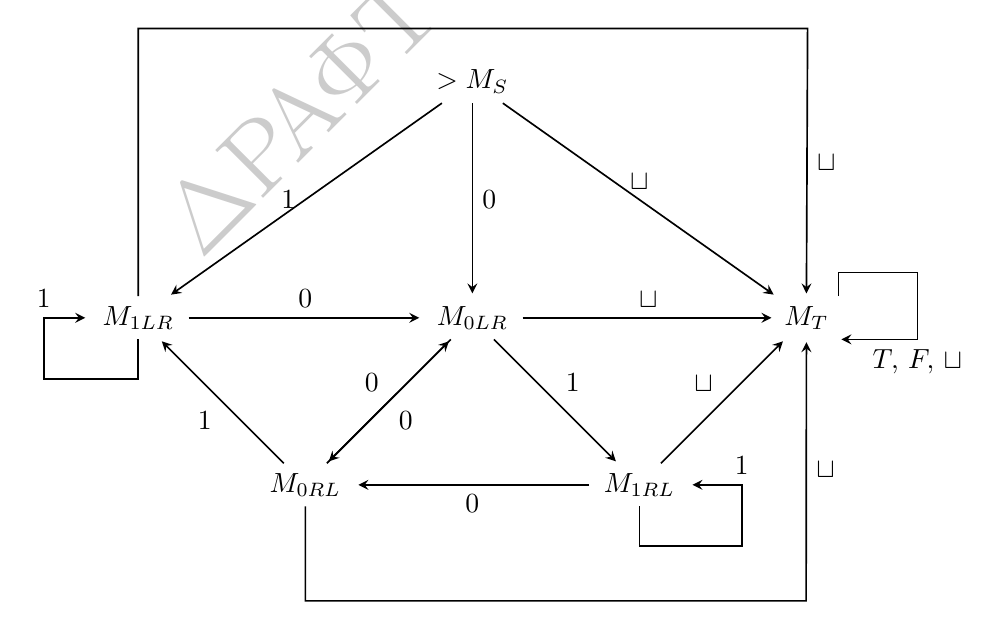
\begin{tikzpicture}[->,>=stealth, shorten >=1pt,semithick,node distance=3.0cm,auto]

		\node(q_1)                  {$\,>M_S\,$};
		\node(q_2) [below of = q_1] {$\,M_{0LR}\,$};
		\node(q_4) [below left of = q_2] {$\,M_{0RL}\,$};
		\node(q_5) [below right of = q_2] {$\,M_{1RL}\,$};
		\node(q_3) [above left of = q_4] {$\,M_{1LR}\,$};
		\node(q_6) [above right of = q_5] {$M_T$};

		\draw[->] (q_1) -- node {$0$} (q_2);
		\draw[->] (q_1) -- node[midway, above] {$\sqcup$} (q_6);
		\draw[->] (q_1) -- node[midway, left] {$1$} (q_3);
		\draw[->] (q_2) -- node {$\sqcup$} (q_6);
		\draw[->] (q_2) -- node {$1$} (q_5);
		\draw[->] (q_2) -- node {$0$} (q_4);
		\draw[->] (q_3) -- node {$0$} (q_2);
		\draw (q_3.south) -- ++(0,-0.5cm) -| ++(-1.2cm,0) |- (q_3.west) node[midway, above] {1};
		\draw (q_3.north) -- ++(0,3.4cm) -| ++(8.5cm,0) -- (q_6.north) node[midway, right] {$\sqcup$};
		\draw[->] (q_5) -- node {$0$} (q_4);
		\draw[->] (q_5) -- node {$\sqcup$} (q_6);
		\draw (q_5.south) -- ++(0,-0.5cm) |- ++(1.3cm,0) |- (q_5.east) node[midway, above] {1};
		\draw[->] (q_4) -- node {$0$} (q_2);
		\draw[->] (q_4) -- node {$1$} (q_3);
		\draw (q_4.south) -- ++(0,-1.2cm) -| ++(6.36cm,0) -- (q_6.south) node[midway, right] {$\sqcup$};
		\draw (q_6.north east) -- ++(0,0.3cm) -| ++(1cm,0) |- (q_6.south east) node[midway, below]
		{$T,\,F,\,\sqcup$};

	\end{tikzpicture}
	\vspace{-0.3cm}
\end{center}
%\clearpage


\begin{tcolorbox}[colback=yellow!15!white, colframe=blue!50!white,
	fonttitle=\bfseries\Large, title = Γραμματική και συντακτικό δένδρο]

\vspace{+0.5cm}
\begin{center}
	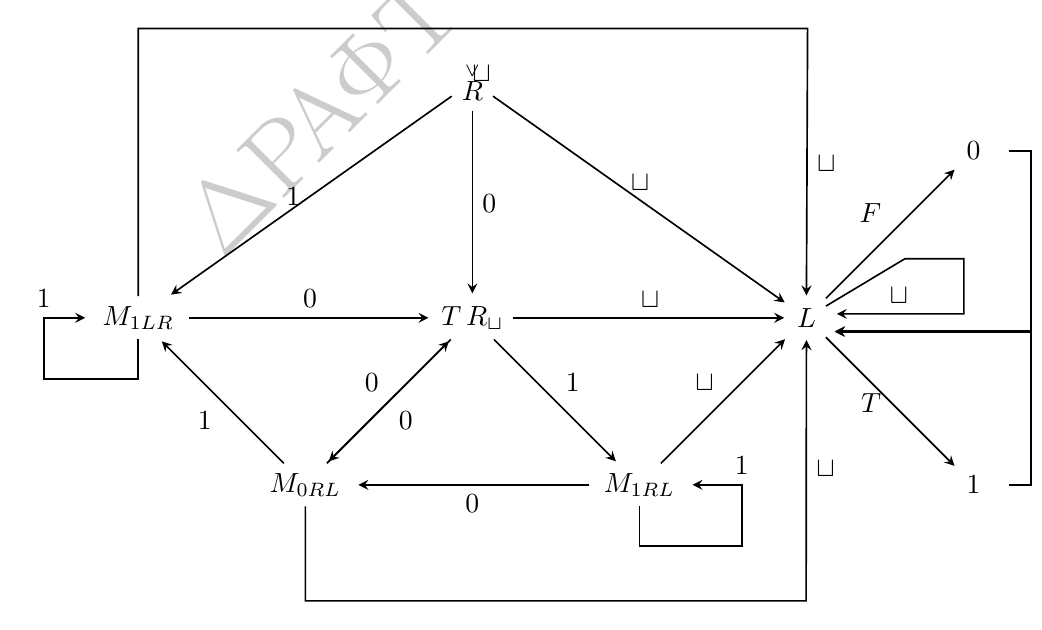
\begin{tikzpicture}[->,>=stealth, shorten >=1pt,semithick,node distance=3.0cm,auto]

		\node(q_1)                  {$\overset{\lor}{R}$};
		\node(q_2) [below of = q_1] {$T\,R_\sqcup$};
		\node(q_4) [below left of = q_2] {$\,M_{0RL}\,$};
		\node(q_5) [below right of = q_2] {$\,M_{1RL}\,$};
		\node(q_3) [above left of = q_4] {$\,M_{1LR}\,$};
		\node(q_6) [above right of = q_5] {$L$};
		\node(q_60) [above right of = q_6] {$0$};
		\node(q_61) [below right of = q_6] {$1$};

		\draw[->] (q_1) -- node {$0$} (q_2);
		\draw[->] (q_1) -- node[midway, above] {$\sqcup$} (q_6);
		\draw[->] (q_1) -- node[midway, left] {$1$} (q_3);
		\draw[->] (q_2) -- node {$\sqcup$} (q_6);
		\draw[->] (q_2) -- node {$1$} (q_5);
		\draw[->] (q_2) -- node {$0$} (q_4);
		\draw[->] (q_3) -- node {$0$} (q_2);
		\draw (q_3.south) -- ++(0,-0.5cm) -| ++(-1.2cm,0) |- (q_3.west) node[midway, above] {1};
		\draw (q_3.north) -- ++(0,3.4cm) -| ++(8.5cm,0) -- (q_6.north) node[midway, right] {$\sqcup$};
		\draw[->] (q_5) -- node {$0$} (q_4);
		\draw[->] (q_5) -- node {$\sqcup$} (q_6);
		\draw (q_5.south) -- ++(0,-0.5cm) |- ++(1.3cm,0) |- (q_5.east) node[midway, above] {1};
		\draw[->] (q_4) -- node {$0$} (q_2);
		\draw[->] (q_4) -- node {$1$} (q_3);
		\draw (q_4.south) -- ++(0,-1.2cm) -| ++(6.36cm,0) -- (q_6.south) node[midway, right] {$\sqcup$};
		\draw[->] (q_6) -- node {$F$} (q_60);
		\draw[->] (q_6) -- node[left] {$T$} (q_61);
		\draw (q_6) -- ++(1.25cm,0.75cm) -- ++(0.75cm,0) -- ++(0,-0.7cm) -- ++(-1.65cm,0) node[midway, above]
		{$\sqcup$}
		(q_6);
		{$\sqcup$};
		\draw[->] (q_60) -- ++(0.5cm,0) -- ++(0,-2.3cm) -- ++(-2.53cm,0) node {} (q_6);
		\draw[->] (q_61) -- ++(0.5cm,0) -- ++(0,1.95cm) -- ++(-2.53cm,0) node {} (q_6);

	\end{tikzpicture}
	\vspace{+0.6cm}
\end{center}


\end{tcolorbox}


\begin{center}
	%\vspace{2em}
	\noindent\rule{\linewidth}{0.5pt}
	%\vspace{2em}
\end{center}
\clearpage
	\newpage
	%\subsection{Απάντηση Υποερωτήματος (γ)}
\label{ssec:Solution_1.3}
\doublespacing
Κανένας περιορισμός για $b$ και $c$ πέρα του ότι θα πρέπει να παρεμβάλετε τουλάχιστον μία εμφάνιση ενός
από αυτά, ανάμεσα σε τυχών δύο συνεχόμενα $a$ και εφόσον\\
$L\! =\! \{w \in \{a,\, b,\, c\}^* \mid (\forall k \in \mathbb{N}^0, \nexists i \in [1\dots \vert w\vert-1])
[\vert w\vert_a = 4k+1,\, w_i = w_{i+1} = a]\}$ άρα $\vert w\vert_{min} = 1$.


%\par
%\phantom{\text{Ελάχιστη περίπτωση}}
\begin{equation*}
		\overset{\text{Ελάχιστη περίπτωση }}{\rightarrow} a
\end{equation*}
\begin{equation*}
	\begin{split}
		\begin{gathered}
	\overset{\vert w \vert_a = 4k+1}{\rightarrow}
	 (aaaa)^* a
	\overset{\text{απεριόριστα }b, c}{\rightarrow}\\
	(b \cup c)^* \; [ a\, (b \cup c)^*\, a\, (b \cup c)^*\, a \,(b \cup c)^*\, a\, (b \cup c)^*]^*\; a\; (b \cup
	c)^* \\
	\overset{\text{όχι συνεχόμενα }a}{\rightarrow}
	(b \cup c)^* \; [a\, (b \cup c)^+\, a\, (b \cup c)^+\, a \,(b \cup c)^+\, a\, (b \cup c)^+]^*\; a \;(b \cup c)^*
		\end{gathered}
	\end{split}
\end{equation*}

\par
Θα τη "σπάσουμε" σε τμήματα χάριν ευκολίας ανάγνωσης:
\reducevspace\reducevspace\reducevspace
\reducevspace\reducevspace\reducevspace
\begin{comment}
	\phantom{\text{Τελική κανονική έκφραση χωρισμένη βάση μοτίβου}}
	\begin{equation*}
		{\boldmath
			\begin{split}
				\begin{gathered}
					(b^*c^*)^*\textcolor{orange}{[}
					\\(a\textcolor{purple}{[}b(b^*c^*)^* \cup c(b^*c^*)^*\textcolor{purple}{]})
					\\(a\textcolor{purple}{[}b(b^*c^*)^* \cup c(b^*c^*)^*\textcolor{purple}{]})
					\\(a\textcolor{purple}{[}b(b^*c^*)^* \cup c(b^*c^*)^*\textcolor{purple}{]})
					\\(a\textcolor{purple}{[}b(b^*c^*)^* \cup c(b^*c^*)^*\textcolor{purple}{]})
					\\ \textcolor{orange}{]}^* a(b^*c^*)^*
				\end{gathered}
		\end{split}}
		\;\;\;\;\;\;\;\;\;\;\text{Τελική κανονική έκφραση χωρισμένη βάση μοτίβου}
	\end{equation*}
\end{comment}

\hfill \break
\mathversion{bold}
\begin{tcolorbox}[colback=yellow!15!white, colframe=blue!50!white,
	fonttitle=\bfseries\Large, title = Κανονική έκφραση χωρισμένη βάση μοτίβου]
	\reducevspace\reducevspace\reducevspace\reducevspace\reducevspace\reducevspace
	\reducevspace\reducevspace\reducevspace\reducevspace\reducevspace\reducevspace
	\begin{align*}
		\begin{gathered}
			(b \cup c)^*\\
			[a\,
			\textcolor{red}{(}b \textcolor{red}{\cup} c\textcolor{red}{)}^+\,
			 a\,
			  \textcolor{red}{(}b \textcolor{red}{\cup} c\textcolor{red}{)}^+\,
			   a \,
			   \textcolor{red}{(}b \textcolor{red}{\cup} c\textcolor{red}{)}^+\,
			    a\,
			    \textcolor{red}{(}b \textcolor{red}{\cup} c\textcolor{red}{)}^+
			     ]^*\;\\
			 a\\
			 (b \cup c)^*
		\end{gathered}
	\end{align*}
\end{tcolorbox}
\mathversion{normal}
\begin{center}
	%\vspace{2em}
	\noindent\rule{\linewidth}{0.5pt}
	%\vspace{2em}
\end{center}
\clearpage
	%\newpage

	\section{Άσκηση 2η - Πεπερασμένα αυτόματα:}
\label{sec:Exercise_2}
\doublespacing

[30\%] Κατασκευάστε αυτόματα στοίβας για τις παρακάτω γλώσσες:

\bm{\textcolor{blue}{(α)}} $L_1 = \{b^n a^k b^k a^n : k, n \in  \mathbb{N}^0 \}$

\bm{\textcolor{blue}{(β)}} $L_2 = \{w \in \{a, b\}^* :  \text{η } w \text{ περιέχει διπλάσιο αριθμό } b
\text{ απ'ότι } a\}$

Για κάθε μία από τις συμβολοσειρές $bbbabaaa \in L_1,\quad abbbab \in L_2$ δώστε έναν υπολογισμό αποδοχής στο
αντίστοιχο αυτόματο στοίβας χρησιμοποιώντας συνολικές καταστάσεις.
\clearpage
	\newpage
	\subsection{Απάντηση Υποερωτήματος (α)}
\label{ssec:Solution_2.1}
\doublespacing
Έχουμε $L = \{w \in \{a,\,b\}^* \;\vert\; (\forall n \in \mathbb{N}^0)\;[\exists w \ni (\bigcup\limits_{k =
|w|-1}^{|w|}w_k = bb \land \vert w \vert = 2n+1\,)\,]\,\}$, \\
όθεν $\vert w\vert_{min} = 3$.\\
 Προς εύρεση αυτομάτου αναγνωρίζων τη δοθέντα γλώσσα το πρόβλημα
θα αποδομηθεί βάση περιορισμών και θα κατασκευασθούν αυτόματα που αναγνωρίζουν έκαστη εκ
των δύο συνθηκών απομονωμένα.

\begin{itemize}
	\itemsep0em
	\item Το 1ο αυτόματο $M_{1}$ θα αναγνωρίζει λέξη περιττού πλήθους χαρακτήρων.
	\item Το 2ο αυτόματο $M_{2}$ θα αναγνωρίζει συμβολοσειρά, λήγουσα σε $bb$.
\end{itemize}

\begin{figure}[!htb]
	\begin{subfigure}{.50\textwidth}
		%\begin{minipage}{0.45\textwidth}
		\centering
		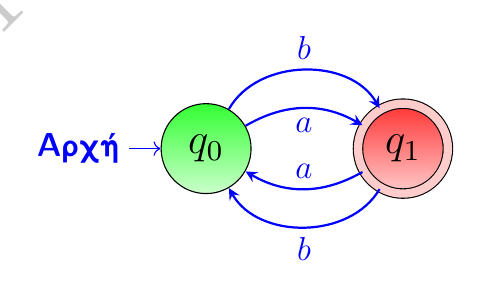
\begin{tikzpicture} [blue, node distance = 2.5cm, on grid, font=\sffamily\large\bfseries]
			% Help grid
			%	\draw [help lines] (-1,4) grid (8,-10);
			% Start Node : Every other node is measured based to this one
			\node (q0) [state, black, scale = 1.3, initial left, initial distance = 4mm, initial text = {Αρχή},
			top color = green!80, bottom color = green!20] {$q_{0}$};
			% Final Node
			\node (q1) [state, black, scale = 1.3, accepting, top color = red!80, bottom color = red!20, double
			distance = 3pt, double = red!20, right = of q0] {$q_{1}$};
			% Draw Arrows/Connections
			\path [-stealth, thick]
			(q0) edge [bend left] node [below] {$a$}(q1)
			(q0) edge [bend left = 60] node [above] {$b$} (q1)
			(q1) edge [bend left] node [above] {$a$} (q0)
			(q1) edge [bend left = 60] node [below] {$b$} (q0);
		\end{tikzpicture}
		%\end{flushleft}
		\caption{DFA $M_{1}$ :\\$L = \{\,w\in \{a, b\}^* \vert\,  \vert w \vert = 2n+1,\, n \in \mathbb{N}^0\}$}
		\label{fig:sub1}
	\end{subfigure}
	\begin{subfigure}{.50\textwidth}
		%\end{minipage}
		%\begin{minipage}{0.45\textwidth}
		\centering
		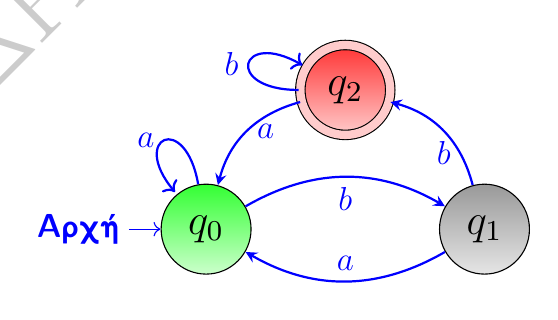
\begin{tikzpicture} [blue, node distance = 2.5cm, on grid, font=\sffamily\large\bfseries]
			% Help grid
			%	\draw [help lines] (-1,4) grid (8,-10);
			% Start Node : Every other node is measured based to this one
			\node (q0) [state, black, scale = 1.3, initial left, initial distance = 4mm, initial text = {Αρχή},
			top color = green!80, bottom color = green!20] {$q_{0}$};

			% Final Node
			\node (q2) [state, black, scale = 1.3, accepting, top color = red!80, bottom color = red!20, double
			distance = 3pt, double = red!20, above right = of q0] {$q_{2}$};

			% Middle Nodes
			\node (q1) [state, black, scale = 1.3, top color = gray!80, bottom color = gray!20, distance = 3pt, below right =
			of q2]
			{$q_{1}$};

			% Draw Arrows/Connections
			\path [-stealth, thick]
			(q0) edge [out = 100, in = 130, loop] node [left] {$a$}(q1)
			(q0) edge [bend left] node [below] {$b$} (q1)
			(q1) edge [bend left] node [above] {$a$} (q0)
			(q1) edge [bend right] node [below] {$b$} (q2)
			(q2) edge [bend right] node [right] {$a$} (q0)
			(q2) edge [out = 180, in = 150,loop] node [left] {$b$} (q2);
		\end{tikzpicture}
		% \end{flushright}
	%\end{minipage}
	\caption{DFA $M_{2}$ :\\$L = \{\,w \in \{a, b\}^* \vert y=bb, \forall x \in \{a, b\}^*, w = xy\}$}
	\label{fig:sub1}
\end{subfigure}
\caption{Αποδόμηση προβλήματος (2-α)} \label{fig:M1}
\end{figure}

\hfill \break

\reducevspace\reducevspace\reducevspace\reducevspace\reducevspace\reducevspace\reducevspace
\reducevspace\reducevspace\reducevspace\reducevspace\reducevspace\reducevspace\reducevspace
\par
Είμαστε έτοιμοι να συνθέσουμε το τελικό αυτόματο $M_{\text{Τ}}$ με $Q_{\text{Τ}} = Q_{1} \bm{\times} Q_{2}
=$\\ $\{(q_1,\, q_2) \;\vert\; q_1 \in Q_1 \in M1, q_2 \in Q_2 \in M2\}$, όθεν επίσης δείχνει ότι έχουμε\\ $\vert
Q_{1}\vert \bm{\cdot} \vert Q_{2}\vert = \vert
Q_{\text{Τ}}\vert_{max} \Longrightarrow 2\bm{\cdot} 3 = 6$:
\clearpage

Κόμβοι:
\reducevspace\reducevspace\reducevspace\reducevspace\reducevspace\reducevspace\reducevspace
\reducevspace\reducevspace\reducevspace\reducevspace\reducevspace\reducevspace\reducevspace
\begin{multicols}{3}
	\begin{itemize}
		\itemsep0em
		\item $q_T^{0} = (q_1^{0}, q_2^{0})$
		\item $q_T^{1} = (q_1^{0}, q_2^{1})$

		\item $q_T^{2} = (q_1^{0}, q_2^{2})$
		\item $q_T^{3} = (q_1^{1}, q_2^{0})$

		\item $q_T^{4} = (q_1^{1}, q_2^{1})$
		\item $q_T^{5} = (q_1^{1}, q_2^{2})$
	\end{itemize}
\end{multicols}
\reducevspace\reducevspace\reducevspace\reducevspace\reducevspace\reducevspace\reducevspace
\par Μεταβάσεις:
\reducevspace\reducevspace\reducevspace\reducevspace\reducevspace\reducevspace\reducevspace
\reducevspace\reducevspace\reducevspace\reducevspace\reducevspace\reducevspace\reducevspace
\begin{multicols}{2}
	\begin{itemize}
		\itemsep0em
		\item $q_T^{0} = (q_1^{0}, q_2^{0}) \bm{\rightarrow^{a}} (q_1^{1}, q_2^{0}) = q_T^{3}$
		\item $q_T^{1} = (q_1^{0}, q_2^{1}) \bm{\rightarrow^{a}} (q_1^{1}, q_2^{0}) = q_T^{3}$
		\item $q_T^{2} = (q_1^{0}, q_2^{2}) \bm{\rightarrow^{a}} (q_1^{1}, q_2^{0}) = q_T^{3}$
		\item $q_T^{3} = (q_1^{1}, q_2^{0}) \bm{\rightarrow^{a}} (q_1^{0}, q_2^{0}) = q_T^{0}$
		\item $q_T^{4} = (q_1^{1}, q_2^{1}) \bm{\rightarrow^{a}} (q_1^{0}, q_2^{0}) = q_T^{0}$
		\item $q_T^{5} = (q_1^{1}, q_2^{2}) \bm{\rightarrow^{a}} (q_1^{0}, q_2^{0}) = q_T^{0}$

		\item $q_T^{0} = (q_1^{0}, q_2^{0}) \bm{\rightarrow^{b}} (q_1^{1}, q_2^{1}) = q_T^{4}$
		\item $q_T^{1} = (q_1^{0}, q_2^{1}) \bm{\rightarrow^{b}} (q_1^{1}, q_2^{2}) = q_T^{5}$
		\item $q_T^{2} = (q_1^{0}, q_2^{2}) \bm{\rightarrow^{b}} (q_1^{1}, q_2^{2}) = q_T^{5}$
		\item $q_T^{3} = (q_1^{1}, q_2^{0}) \bm{\rightarrow^{b}} (q_1^{0}, q_2^{1}) = q_T^{1}$
		\item $q_T^{4} = (q_1^{1}, q_2^{1}) \bm{\rightarrow^{b}} (q_1^{0}, q_2^{2}) = q_T^{2}$
		\item $q_T^{5} = (q_1^{1}, q_2^{2}) \bm{\rightarrow^{b}} (q_1^{0}, q_2^{2}) = q_T^{2}$
	\end{itemize}
\end{multicols}
\reducevspace\reducevspace\reducevspace\reducevspace\reducevspace\reducevspace\reducevspace
\reducevspace\reducevspace\reducevspace\reducevspace\reducevspace\reducevspace\reducevspace
\par
Έχουμε DFA $M_{\text{Τ}}$ με εξής μη ενδιαμέσους κόμβους:\\
αρχικό $s_{\text{Τ}} \in M_{\text{Τ}} = \{(q_1,\, q_2) \;\vert\; q_1 = s_1 \in M_1, q_2 = s_2 \in M_2 \}
\Longrightarrow q_{\text{Τ}}^0 = {q_1^0, q_2^0}$,\\
τελικό $F_{\text{Τ}}\in M_{\text{Τ}} =\{(q_1,\, q_2) \;\vert\; q_1\in F_1 \in M_1, q_2\in F_2\in M_2 \}
\Longrightarrow q_{\text{Τ}}^5 = {q_1^1, q_2^2}$\\
\hfill \break
DFA $ M_{\text{Τ}} = (\; \{\,q0,\, q1,\, q2,\, q3,\, q4,\, q5\,\}, \{\,a,\, b\,\},\\
\{\,δ(q0,\, a)=q3,\, δ(q0, b)=q4,\, δ(q1, a)=q3,\, δ(q1, b)=q5,\\
δ(q2, a)=q3,\, δ(q2, b)=q5,\, δ(q3, a)=q0,\, δ(q3, b)=q1,\\
δ(q4, a)=q0,\, δ(q4, b)=q2,\, δ(q5, a)=q0,\, δ(q5, b)=q2\,\},\\
q0,\; \{\,q5\,\}\;)$


\hfill \break
\begin{tcolorbox}[colback=yellow!15!white, colframe=blue!50!white,
	fonttitle=\bfseries\Large, title = DFA $M_{\text{Τ}}$]
%\begin{figure}[!htb]
		\centering
		%\begin{minipage}{0.45\textwidth}
		%\begin{flushleft}
		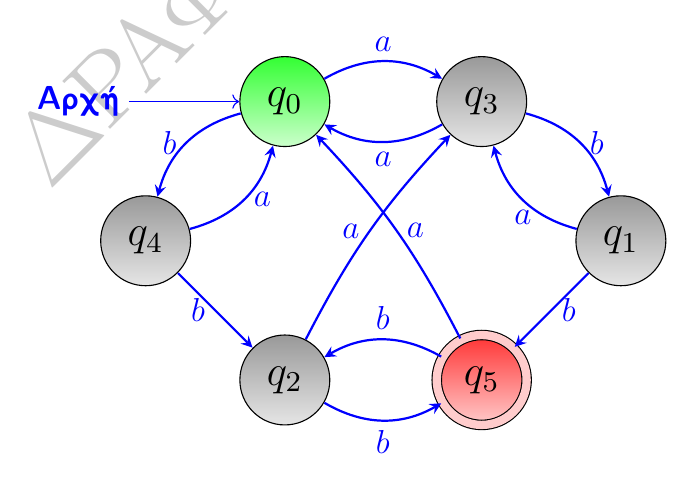
\begin{tikzpicture} [blue, node distance = 2.5cm, on grid, font=\sffamily\large\bfseries]
			% Help grid
			%	\draw [help lines] (-1,4) grid (8,-10);
			% Start Node : Every other node is measured based to this one
			\node (q0) [state, black, scale = 1.3, initial left, initial distance = 14mm, initial text = {Αρχή},
			top color = green!80, bottom color = green!20] {$q_{0}$};

			\node (q3) [state, black, scale = 1.3, top color = gray!80, bottom color = gray!20, distance = 3pt, right = of
			q0]
			{$q_{3}$};

			\node (q1) [state, black, scale = 1.3, top color = gray!80, bottom color = gray!20, distance = 3pt,
			below right = of q3] {$q_{1}$};

			\node (q4) [state, black, scale = 1.3, top color = gray!80, bottom color = gray!20, distance = 3pt, below left =
			of q0]
			{$q_{4}$};

			\node (q2) [state, black, scale = 1.3, top color = gray!80, bottom color = gray!20, distance = 3pt, below right =
			of q4]
			{$q_{2}$};

			% Final Node
			\node (q5) [state, black, scale = 1.3, accepting, top color = red!80, bottom color = red!20, double
			distance = 3pt, double = red!20, right = of q2] {$q_{5}$};
			% Draw Arrows/Connections
			\path [-stealth, thick]

			% 0,0 => 1,0 || 1,1
			(q0) edge [bend left] node [above] {$a$}(q3)
			(q0) edge [bend right] node [left] {$b$} (q4)
			% 0,1 => 1,0 || 1,2
			(q1) edge [bend left] node [below] {$a$} (q3)
			(q1) edge [] node [right] {$b$} (q5)
			% 0,2 => 1,0 || 1,2
			(q2) edge [bend left = 8] node [left] {$a$} (q3)
			(q2) edge [bend right] node [below] {$b$} (q5)
			% 1,0 => 0,0 || 0,1
			(q3) edge [bend left] node [below] {$a$} (q0)
			(q3) edge [bend left] node [right] {$b$} (q1)
			% 1,1 => 0,0 || 0,2
			(q4) edge [bend right] node [right] {$a$} (q0)
			(q4) edge [] node [left] {$b$} (q2)
			% 1,2 => 0,0 || 0,2
			(q5) edge [bend right = 8] node [right] {$a$} (q0)
			(q5) edge [bend right] node [above] {$b$} (q2);
		\end{tikzpicture}
%		\caption{DFA $M_{1}$ : \\ $L = \{\,w\; \vert \; (w \in \{a, b\}^*) \; [\vert w \vert$ περιττό$]\}$}
%		\label{fig:sub1}
%\end{figure}

\end{tcolorbox}
\begin{center}
	%\vspace{2em}
	\noindent\rule{\linewidth}{0.5pt}
	%\vspace{2em}
\end{center}

\clearpage
	\newpage
	\subsection{Απάντηση Υποερωτήματος (β)}
\label{ssec:Solution_2.2}
\doublespacing
Έχουμε να κατασκευάσουμε PDA για CFL $L_1 = \{b^n a^k b^k a^n : k, n \in  \mathbb{N}^0 \}$\\
Από τον τύπο δυνάμεθα να εξάγουμε τα εξής δεδομένα, για συμβολοσειρά $w \in L_1$:
\reducevspace\reducevspace\reducevspace\reducevspace\reducevspace\reducevspace
\begin{itemize}
	\itemsep0em
	\item $\vert w \vert_{min} = 0 \Longrightarrow n,\,k = 0 \Longrightarrow w = ε$, \quad $\vert w \vert_{max} =
	\aleph_0$, \quad $|w| = 2(n+k) = \text{Άρτιο}$
	\item $ n + k - 2nk = 1  \Longrightarrow |w|_{min} = 2 \Longrightarrow w = ba \cup ab$
	\item $ n, k = 1 \Longrightarrow \vert w \vert_{min} = 4 \Longrightarrow w = baba$, \qquad $L \subseteq \{xx^R
	\vert x \in \Sigma^* \}$
	\item Για μεγαλύτερα $n, k$ έχουμε συμβολοσειρές όπως $bbabaa, baabba, bbaabbaa...$
\end{itemize}
\reducevspace\reducevspace
\par
Από αυτά κάποια δεν μας λένε κάτι ιδιαίτερα χρήσιμο, άλλα όμως μας φανερώνουν την οδό που θα πρέπει να
ακολουθήσουμε. Για παράδειγμα, κατά αντιστοιχία με τις αντίστοιχες τεχνικές που ακολουθήσαμε στις
λύσεις ασκήσεων κανονικών εκφράσεων, τα διάφορα ελάχιστα μας δίνουν την βάση πάνω στην οποία θα χτιστεί το (PD)
αυτόματο.
\par
Ως εκ τούτου έχουμε φαινομενικά τέσσερεις ελάχιστες περιπτώσεις, που η
συγκεκριμένη γλώσσα επιτρέπει:
$w_0 = ε \lor w_1 = ab \lor w_2 = ba \lor w_3 = baba$ αλλά προσοχή, το $w = baba$
αποτελεί παρεμβολή του $w_1$ εντός του $w_2$ και όχι $(ba)^*$
\par
Αυτό με τη σειρά του δείχνει ότι ουσιαστικά, το $w_3$ αποτελεί επέκταση της $w_2$ μετά αρχικού $b$ και άρα δεν
είναι μέρος της καθολικής βάσης του αυτομάτου. Θα μας χρειαστεί όμως, αφού δείχνει ότι όταν ο
αλγόριθμος θα μπαίνει στη διαδρομή που διαβάζει $ba$, θα διακλαδώνεται σε δύο εναλλακτικές βάση του
αν αυτό που έπεται του $b$ είναι $a$ ή $aba$.
\par Τέλος αφού $n, k \in \mathbb{N_0}$ τότε μπορούν όλοι αυτοί οι χαρακτήρες να είναι (μετρήσιμα) άπειροι αλλά υπό
τον όρο ότι τηρείται το γενικό μοτίβο.
\par Άρα, θεωρητικά, έχουμε 3 αρχικούς κλάδους και  και σε έναν από αυτούς άλλη μία διάσπαση σε δύο. Θα δούμε
τελικά ότι ακριβώς αυτό συμβαίνει και στην πράξη (τουλάχιστον στη συγκεκριμένη επίλυση) και ότι γενικά είναι καλή
πρακτική. Ξεκινάμε την κατασκευή του αυτομάτου, αρχικά δίνοντας την μαθηματική περιγραφή και κατόπιν το αντίστοιχο
διάγραμμα:

\begin{tcolorbox}[colback=yellow!15!white, colframe=blue!50!white,
	fonttitle=\bfseries\Large, title = {PDA $M = (K,\, \Sigma,\, \Gamma,\, \Delta,\, s,\, F)$}]
\begin{itemize}
	\itemsep0em
	\item $K \,=\, \{q1,\, q2,\, q3,\, q4,\, q5,\, q6\}$
	\item $\Sigma \,=\, \{a,\, b\}$
	\item $\Gamma \,=\, \{A,\, B,\, \$\}$
	\item $\Delta \,=\,$
	\reducevspace\reducevspace\reducevspace\reducevspace\reducevspace\reducevspace\reducevspace
	\reducevspace\reducevspace\reducevspace\reducevspace\reducevspace\reducevspace\reducevspace
		\begin{multicols}{2}
		\begin{enumerate}
			\item $(q1,\,ε,\,ε)\rightarrow(q2,\,\$)$



			\item $(q2,\,b,\,\$)\rightarrow(q2,\,B\$)$
			\item $(q2,\,b,\,B)\rightarrow(q2,\,BB)$

			\item $(q2,\,ε,\,\$)\rightarrow(q6,\,ε)$
			\item $(q2,\,a,\,\$)\rightarrow(q3,\,A\$)$
			\item $(q2,\,a,\,B)\rightarrow(q3,\,AB)$
			\item $(q2,\,a,\,B)\rightarrow(q5,\,ε)$



			\item $(q3,\,a,\,A)\rightarrow(q3,\,AA)$

			\item $(q3,\,b,\,A)\rightarrow(q4,\,ε)$



			\item $(q4,\,b,\,A)\rightarrow(q1,\,ε)$

			\item $(q4,\,a,\,B)\rightarrow(q5,\,ε)$
			\item $(q4,\,ε,\,\$)\rightarrow(q6,\,ε)$



			\item $(q5,\,a,\,B)\rightarrow(q5,\,ε)$

			\item $(q5,\,ε,\,\$)\rightarrow(q6,\,ε)$
		\end{enumerate}
		\end{multicols}
	\item $s \,=\, q_1$
	\item $F \,=\, q_6$
\end{itemize}
\end{tcolorbox}
\reducevspace\reducevspace\reducevspace\reducevspace\reducevspace\reducevspace\reducevspace

%\par
\begin{comment}
\begin{figure}[!htb]
	\centering
	%\begin{minipage}{0.45\textwidth}
	%\begin{flushleft}
	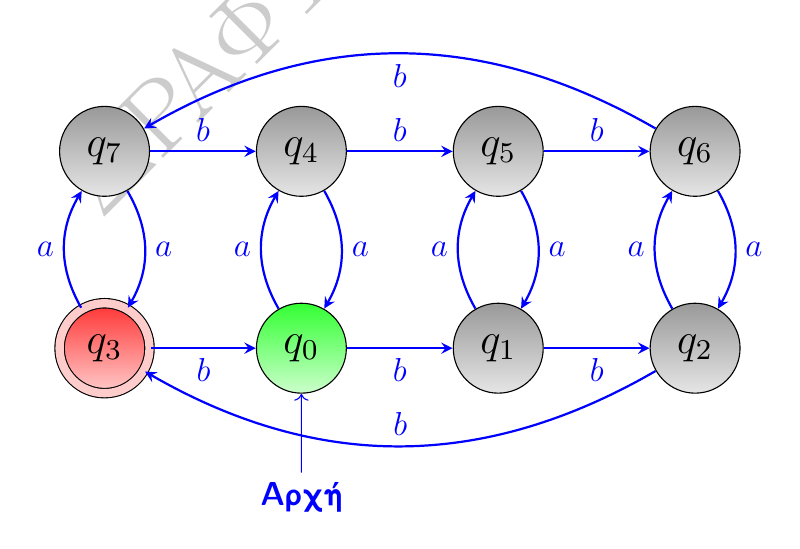
\begin{tikzpicture} [blue, node distance = 2.5cm, on grid, font=\sffamily\large\bfseries]
		% Help grid
		%	\draw [help lines] (-1,4) grid (8,-10);
		% Start Node : Every other node is measured based to this one
		\node (q0) [state, black, scale = 1.3, initial below, initial distance = 10mm, initial text = {Αρχή},
		top color = green!80, bottom color = green!20] {$q_{0}$};

		% Final Node
		\node (q3) [state, black, scale = 1.3,accepting, top color = red!80, bottom color = red!20, double
		distance = 3pt, double = red!20, left = of q0] {$q_{3}$};

		\node (q1) [state, black, scale = 1.3, top color = gray!80, bottom color = gray!20, right = of q0] {$q_{1}$};

		\node (q2) [state, black, scale = 1.3, top color = gray!80, bottom color = gray!20, right = of q1] {$q_{2}$};

		\node (q4) [state, black, scale = 1.3, top color = gray!80, bottom color = gray!20, above = of q0] {$q_{4}$};

		\node (q5) [state, black, scale = 1.3, top color = gray!80, bottom color = gray!20, right = of q4] {$q_{5}$};

		\node (q6) [state, black, scale = 1.3, top color = gray!80, bottom color = gray!20, right = of q5] {$q_{6}$};

		\node (q7) [state, black, scale = 1.3, top color = gray!80, bottom color = gray!20, left = of q4] {$q_{7}$};

		% Draw Arrows/Connections
		\path [-stealth, thick]

		% 0,0 => 1,0 || 0,1
		(q0) edge [bend left] node [left] {$a$}(q4)
		(q0) edge [] node [below] {$b$} (q1)
		% 0,1 => 1,1 || 0,2
		(q1) edge [bend left] node [left] {$a$} (q5)
		(q1) edge [] node [below] {$b$} (q2)
		% 0,2 => 1,2 || 0,3
		(q2) edge [bend left] node [left] {$a$} (q6)
		(q2) edge [bend left] node [above] {$b$} (q3)
		% 0,3 => 1,3 || 0,0
		(q3) edge [bend left] node [left] {$a$} (q7)
		(q3) edge [] node [below] {$b$} (q0)
		% 1,0 => 0,0 || 1,1
		(q4) edge [bend left] node [right] {$a$} (q0)
		(q4) edge [] node [above] {$b$} (q5)
		% 1,1 => 0,1 || 1,2
		(q5) edge [bend left] node [right] {$a$} (q1)
		(q5) edge [] node [above] {$b$} (q6)
		% 1,2 => 0,2 || 1,3
		(q6) edge [bend left] node [right] {$a$} (q2)
		(q6) edge [bend right] node [below] {$b$} (q7)
		% 1,3 => 0,3 || 1,0
		(q7) edge [bend left] node [right] {$a$} (q3)
		(q7) edge [] node [above] {$b$} (q4);
	\end{tikzpicture}
	\caption{DFA $M_{1}$ : \\ $L = \{\,w\; \vert \; (w \in \{a, b\}^*) \; [\vert w \vert$ περιττό$]\}$}
	\label{fig:sub1}
\end{figure}
\end{comment}

%\vfill
%\clearpage
\begin{tcolorbox}[colback=yellow!15!white, colframe=blue!50!white,
	fonttitle=\bfseries\Large, title = DFA $M_{\text{τελικό}}$]
	\centering
	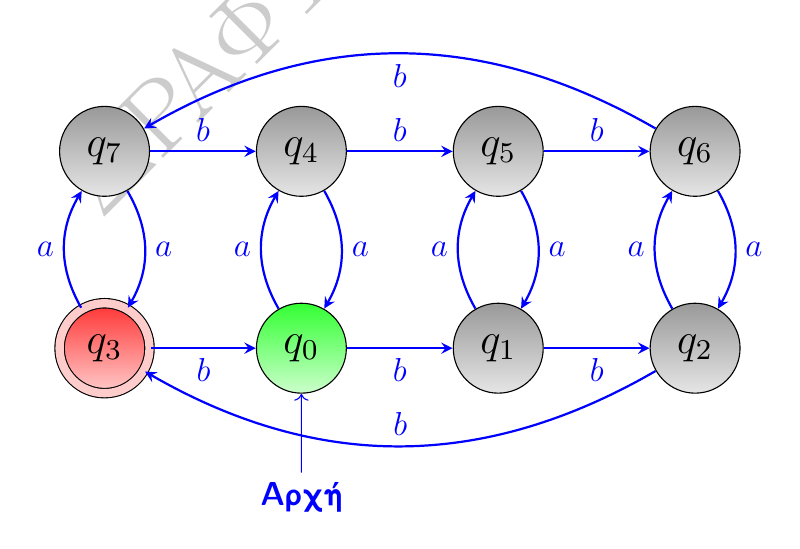
\begin{tikzpicture} [blue, node distance = 2.5cm, on grid, font=\sffamily\large\bfseries]
		% Help grid
		%	\draw [help lines] (-1,4) grid (8,-10);
		% Start Node : Every other node is measured based to this one
		\node (q0) [state, black, scale = 1.3, initial below, initial distance = 10mm, initial text = {Αρχή},
		top color = green!80, bottom color = green!20] {$q_{0}$};

		% Final Node
		\node (q3) [state, black, scale = 1.3,accepting, top color = red!80, bottom color = red!20, double
		distance = 3pt, double = red!20, left = of q0] {$q_{3}$};

		\node (q1) [state, black, scale = 1.3, top color = gray!80, bottom color = gray!20, right = of q0]
		{$q_{1}$};

		\node (q2) [state, black, scale = 1.3, top color = gray!80, bottom color = gray!20, right = of q1]
		{$q_{2}$};

		\node (q4) [state, black, scale = 1.3, top color = gray!80, bottom color = gray!20, above = of q0]
		{$q_{4}$};

		\node (q5) [state, black, scale = 1.3, top color = gray!80, bottom color = gray!20, right = of q4]
		{$q_{5}$};

		\node (q6) [state, black, scale = 1.3, top color = gray!80, bottom color = gray!20, right = of q5]
		{$q_{6}$};

		\node (q7) [state, black, scale = 1.3, top color = gray!80, bottom color = gray!20, left = of q4] {$q_{7}$};

		% Draw Arrows/Connections
		\path [-stealth, thick]

		% 0,0 => 1,0 || 0,1
		(q0) edge [bend left] node [left] {$a$}(q4)
		(q0) edge [] node [below] {$b$} (q1)
		% 0,1 => 1,1 || 0,2
		(q1) edge [bend left] node [left] {$a$} (q5)
		(q1) edge [] node [below] {$b$} (q2)
		% 0,2 => 1,2 || 0,3
		(q2) edge [bend left] node [left] {$a$} (q6)
		(q2) edge [bend left] node [above] {$b$} (q3)
		% 0,3 => 1,3 || 0,0
		(q3) edge [bend left] node [left] {$a$} (q7)
		(q3) edge [] node [below] {$b$} (q0)
		% 1,0 => 0,0 || 1,1
		(q4) edge [bend left] node [right] {$a$} (q0)
		(q4) edge [] node [above] {$b$} (q5)
		% 1,1 => 0,1 || 1,2
		(q5) edge [bend left] node [right] {$a$} (q1)
		(q5) edge [] node [above] {$b$} (q6)
		% 1,2 => 0,2 || 1,3
		(q6) edge [bend left] node [right] {$a$} (q2)
		(q6) edge [bend right] node [below] {$b$} (q7)
		% 1,3 => 0,3 || 1,0
		(q7) edge [bend left] node [right] {$a$} (q3)
		(q7) edge [] node [above] {$b$} (q4);
	\end{tikzpicture}
\end{tcolorbox}
\begin{center}
	%\vspace{2em}
	\noindent\rule{\linewidth}{0.5pt}
	%\vspace{2em}
\end{center}
%\clearpage

	\hfill \break
	\newpage
	%\subsection{Απάντηση Υποερωτήματος (γ)}
\label{ssec:Solution_2.3}
\doublespacing
Έχουμε $L = \{ w = xy \in \{a, b\}^* \; \vert \; (x \in \{a, b\},\, [\,\vert w\vert_x = 4n+2,\, n \in
\mathbb{N}^0\,]\}$.

\par
Παρατηρούμε ότι ουσιαστικά έχουμε μόνο μία συνθήκη, η οποία ναι μεν ισχύει για όλα τα σύμβολα της γλώσσας αλλά
περιορίζει μόνο ένα από αυτά τη φορά. Αναλυτικότερα, απαιτεί
συγκεκριμένο αριθμό εμφανίσεων του πρώτου συμβόλου, χωρίς όμως να μας ενδιαφέρει οποιοδήποτε άλλο σύμβολο και χωρίς
να μας απασχολούν οι θέσεις τους.

Άρα μη αρχικό σύμβολο δύναται να παρεμβάλλεται παντού εκτός της 1ης θέσης στη λέξη κατά Kleene star
φορές έκαστη.

Επίσης, εφόσον μόνο ο 1ος χαρακτήρας καθορίζει την αναγνωρισιμότητα της λέξης κατά
αποκλειστικότητα, μπορούμε να εξάγουμε άλλα δύο δεδομένα:

\begin{itemize}
	\itemsep0em
	\item Οι κόμβοι του αυτομάτου σχηματίζουν $k = \{\Sigma \in L \;\vert\; \vert\Sigma\vert\}$ αλυσίδες έκαστη
	διαφορετικού
	συμβόλου του αλφαβήτου της γλώσσας, το οποίο δίνει τις μεταβάσεις μεταξύ κόμβων (και τα υπόλοιπα πάνε στις
	λούπες). Κατά άλλα οι "αλυσίδες" είναι ίδιες και με κοινή αφετηρία την αρχική κατάσταση και η αρχική είναι η
	μόνη κατάσταση που μπορούμε να μεταβούμε προς άλλη με οποιοδήποτε σύμβολο.

	\item Ο αρχικός κόμβος, είναι κοινός για όλες τις "αλυσίδες" και δεν περιέχει καμία λούπα ή επιστροφή προς
	αυτόν.

\end{itemize}

%\vfill
%\clearpage
Θα μπορούσαμε να βρούμε το συγκεκριμένο αυτόματο με αποδόμηση όπως και τα προηγούμενα αλλά θα απαιτούσε περιττά
πολύ χρόνο και κόπο, λόγο περιπλοκότητας, άρα:

%\hfill \break
\begin{tcolorbox}[colback=yellow!15!white, colframe=blue!50!white,
	fonttitle=\bfseries\Large, title = Τελικό DFA $M_{\text{τελικό}}$]
	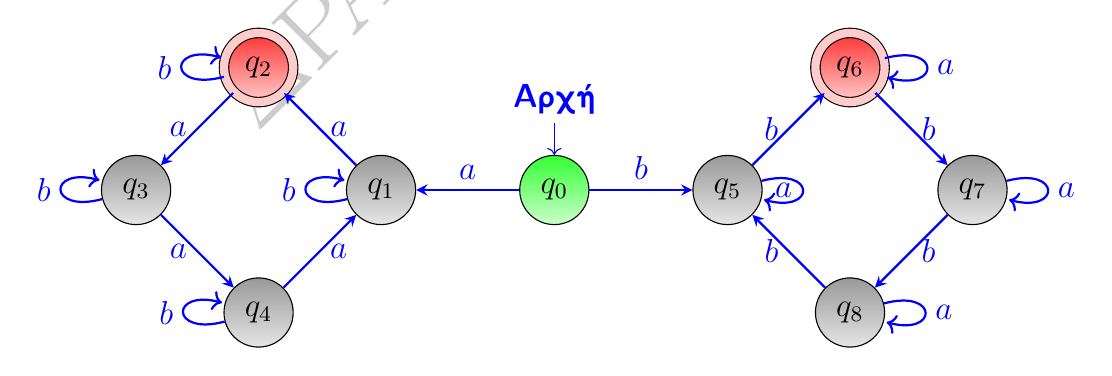
\begin{tikzpicture} [blue, node distance = 2.2cm, on grid, font=\sffamily\large\bfseries]
		% Help grid
		%	\draw [help lines] (-1,4) grid (8,-10);
		% Start Node : Every other node is measured based to this one
		\node (q0) [state, black, scale = 1, initial above, initial distance = 4mm, initial text = {Αρχή},
		top color = green!80, bottom color = green!20] {$q_{0}$};

		% Middle Nodes
		\node (q1) [state, black, scale = 1, top color = gray!80, bottom color = gray!20, left = of q0] {$q_{1}$};
		\node (q4) [state, black, scale = 1, top color = gray!80, bottom color = gray!20, below left = of q1]
		{$q_{4}$};
		\node (q3) [state, black, scale = 1, top color = gray!80, bottom color = gray!20, above left = of q4]
		{$q_{3}$};

		\node (q5) [state, black, scale = 1, top color = gray!80, bottom color = gray!20, right = of q0]
		{$q_{5}$};
		\node (q8) [state, black, scale = 1, top color = gray!80, bottom color = gray!20, below right = of q5]
		{$q_{8}$};
		\node (q7) [state, black, scale = 1, top color = gray!80, bottom color = gray!20, above right = of q8]
		{$q_{7}$};

		% Final Node
		\node (q2) [state, black, scale = 1, accepting, top color = red!80, bottom color = red!20, , double
		distance = 3pt, double = red!20, above left = of q1] {$q_{2}$};

		\node (q6) [state, black, scale = 1, accepting, top color = red!80, bottom color = red!20, , double
		distance = 3pt, double = red!20, above right = of q5] {$q_{6}$};

		% Draw Arrows/Connections
		\path [-stealth, thick]
		(q0) edge [] node [above] {$a$}(q1)
		(q0) edge [] node [above] {$b$} (q5)

		(q1) edge [] node [right] {$a$} (q2)
		(q1) edge [loop left] node [left] {$b$} (q1)
		(q2) edge [] node [left] {$a$} (q3)
		(q2) edge [loop left] node [left] {$b$} (q2)
		(q3) edge [] node [left] {$a$} (q4)
		(q3) edge [loop left] node [left] {$b$} (q3)
		(q4) edge [] node [right] {$a$} (q1)
		(q4) edge [loop left] node [left] {$b$} (q4)

		(q5) edge [loop right] node [left] {$a$} (q5)
		(q5) edge [] node [left] {$b$} (q6)
		(q6) edge [loop right] node [right] {$a$} (q6)
		(q6) edge [] node [right] {$b$} (q7)
		(q7) edge [loop right] node [right] {$a$} (q7)
		(q7) edge [] node [right] {$b$} (q8)
		(q8) edge [loop right] node [right] {$a$} (q8)
		(q8) edge [] node [left] {$b$} (q5);
	\end{tikzpicture}
\end{tcolorbox}
\begin{center}
	%\vspace{2em}
	\noindent\rule{\linewidth}{0.5pt}
	%\vspace{2em}
\end{center}
\clearpage

	\section{Άσκηση 3η - Γλώσσες χωρίς συμφραζόμενα}
\label{sec:Exercise_3}
\doublespacing

\bm{\textcolor{blue}{(α) [5\%]}} Αποφανθείτε αν ο παρακάτω ισχυρισμός είναι σωστός ή λανθασμένος και αιτιολογήστε:
Η τομή μίας ντετερμινιστικής γλώσσας χωρίς συμφραζόμενα με μία πεπερασμένη γλώσσα είναι πάντα γλώσσα χωρίς
συμφραζόμενα.

\bm{\textcolor{blue}{(β) [5\%]}} Αποδείξτε εάν η παρακάτω γλώσσα είναι ή δεν είναι γλώσσα χωρίς συμφραζόμενα:\\
\[L = \{a^mb^nc^k\,:\,n,\,k,\,m\in\mathbb{N}_0,\, n=3m+2k\}\]




\hfill \break


\clearpage
	\newpage
	\subsection{Απάντηση Υποερωτήματος (α)}
\label{ssec:Solution_3.1}
\doublespacing
Η πρόταση "η τομή μίας ντετερμινιστικής γλώσσας χωρίς συμφραζόμενα με μία πεπερασμένη γλώσσα είναι πάντα γλώσσα
χωρίς συμφραζόμενα" είναι αληθής όπως θα αποδείξουμε παρακάτω:


\reducevspace\reducevspace\reducevspace


\begin{tcolorbox}[colback=yellow!15!white, colframe=blue!50!white,
	fonttitle=\bfseries\Large, title = Απόδειξη]
	\centering
\begin{itemize}
	\itemsep0em

	\item $\mathcal{P} := \{\forall\,L_{DCF}\in\mathcal L_{\mathrm{DCF}},\;\forall\,L_{REG}\in\mathcal
	L_{\mathrm{REG}}:\;L_{DCF}\cap L_{REG}\;\in\;\mathcal L_{\mathrm{CF}}\}$
	\reducevspace\reducevspace\reducevspace\reducevspace\reducevspace\reducevspace
	\reducevspace\reducevspace\reducevspace\reducevspace\reducevspace\reducevspace
	\reducevspace\reducevspace\reducevspace\reducevspace\reducevspace\reducevspace
	\reducevspace\reducevspace\reducevspace\reducevspace\reducevspace\reducevspace
	\begin{flushright}\hypertarget{3.1.1}{\bf{(1)}}\end{flushright}


	\item $\mathcal{L}_{FIN} \subset \mathcal{L}_{REG} \subset \mathcal{L}_{DCF} \subset \mathcal{L}_{NCF} =
	\mathcal{L}_{CF}$
	\reducevspace\reducevspace\reducevspace\reducevspace\reducevspace\reducevspace
	\reducevspace\reducevspace\reducevspace\reducevspace\reducevspace\reducevspace
	\reducevspace\reducevspace\reducevspace\reducevspace\reducevspace\reducevspace
	\reducevspace\reducevspace\reducevspace\reducevspace\reducevspace\reducevspace
	\begin{flushright}\hypertarget{3.1.2}{\bf{(2)}}\end{flushright}

	\item $A \subset B \Rightarrow A \cap B = A \subset B$
	\reducevspace\reducevspace\reducevspace\reducevspace\reducevspace\reducevspace
	\reducevspace\reducevspace\reducevspace\reducevspace\reducevspace\reducevspace
	\reducevspace\reducevspace\reducevspace\reducevspace\reducevspace\reducevspace
	\reducevspace\reducevspace\reducevspace\reducevspace\reducevspace\reducevspace
	\begin{flushright}\hypertarget{3.1.3}{\bf{(3)}}\end{flushright}

	\item $A \subset B \subset...\subset N \Rightarrow A \subset N$
	\reducevspace\reducevspace\reducevspace\reducevspace\reducevspace\reducevspace
	\reducevspace\reducevspace\reducevspace\reducevspace\reducevspace\reducevspace
	\reducevspace\reducevspace\reducevspace\reducevspace\reducevspace\reducevspace
	\reducevspace\reducevspace\reducevspace\reducevspace\reducevspace\reducevspace
	\begin{flushright}\hypertarget{3.1.4}{\bf{(4)}}\end{flushright}

	\item $\overset{\hyperlink{3.1.2}{(2)} \hyperlink{3.1.4}{(4)}}{\Longrightarrow} \mathcal{L}_{FIN} \subset
	\mathcal{L}_{DCF}$
	\reducevspace\reducevspace\reducevspace\reducevspace\reducevspace\reducevspace
	\reducevspace\reducevspace\reducevspace\reducevspace\reducevspace\reducevspace
	\reducevspace\reducevspace\reducevspace\reducevspace\reducevspace\reducevspace
	\reducevspace\reducevspace\reducevspace\reducevspace\reducevspace\reducevspace
	\begin{flushright}\hypertarget{3.1.5}{\bf{(5)}}\end{flushright}

	\item $\mathcal{L}_{FIN} \cap \mathcal{L}_{DCF}\!\!\overset{\hyperlink{3.1.3}{(3)}\hyperlink{3.1.5}{(5)}}{=}\!\!
	\mathcal{L}_{FIN} \subset \mathcal{L}_{DCF} \subset \mathcal{L}_{CF}
	\overset{\hyperlink{3.1.4}{(4)}}{\Rightarrow} \mathcal{L}_{FIN} \subset \mathcal{L}_{CF} \Rightarrow
	\mathcal{L}_{FIN} \in \mathcal{L}_{CF}$
	\reducevspace\reducevspace\reducevspace\reducevspace\reducevspace\reducevspace
	\reducevspace\reducevspace\reducevspace\reducevspace\reducevspace\reducevspace
	\reducevspace\reducevspace\reducevspace\reducevspace\reducevspace\reducevspace
	\reducevspace\reducevspace\reducevspace\reducevspace\reducevspace\reducevspace
	\begin{flushright}\hypertarget{3.1.6}{\bf{(6)}}\end{flushright}

	\item $\mathcal{Q} \overset{\hyperlink{3.1.6}{(6)}}{:=} \{\forall\,L_{DCF}\in\mathcal
	L_{\mathrm{DCF}},\;\forall\,L_{REG}\in\mathcal
	L_{\mathrm{REG}}:\;L_{DCF}\cap L_{REG}\;\in\;\mathcal L_{\mathrm{CF}}\}$
	\reducevspace\reducevspace\reducevspace\reducevspace\reducevspace\reducevspace
	\reducevspace\reducevspace\reducevspace\reducevspace\reducevspace\reducevspace
	\reducevspace\reducevspace\reducevspace\reducevspace\reducevspace\reducevspace
	\reducevspace\reducevspace\reducevspace\reducevspace\reducevspace\reducevspace
	\begin{flushright}\hypertarget{3.1.7}{\bf{(7)}}\end{flushright}

	\item $\mathcal{P}^{\hyperlink{3.1.1}{(1)}} = \mathcal{Q}^{\hyperlink{3.1.7}{(7)}} = $ True $ \Rightarrow
	\mathcal{P} = $ True
\end{itemize}
\end{tcolorbox}

\begin{center}
	%\vspace{2em}
	\noindent\rule{\linewidth}{0.5pt}
	%\vspace{2em}
\end{center}
\clearpage
	\newpage
	\subsection{Απάντηση Υποερωτήματος (β)}
\label{ssec:Solution_3.2}
\doublespacing

Η άσκηση μας ζητά να αποδείξουμε εάν η παρακάτω γλώσσα είναι CF ή όχι:
\[L = \{a^mb^nc^k\,:\,n,\,k,\,m\in\mathbb{N}_0,\, n=3m+2k\}\]

\par
Υπάρχουν πάρα πολλοί τρόποι να το κάνουμε αυτό. Μεταξύ των οποίων είναι η απόπειρα κατασκευής CFG της γλώσσας, όπου
αν τα καταφέρουμε αυτόματα αποδεικνύουμε ότι είναι CFL, ενώ μία άλλη μέθοδος είναι μέσω λήμματος άντλησης. Υπάρχουν
αρκετοί ακόμη μέθοδοι αλλά δεν θα τις αναφέρουμε ούτε θα τις δείξουμε όλες.

\begin{tcolorbox}[colback=yellow!15!white, colframe=blue!50!white,
	fonttitle=\bfseries\Large, title = Απόδειξη - μέρος 1/3]
	\begin{itemize}
		\itemsep1em




	\end{itemize}
\end{tcolorbox}


\begin{center}
	%\vspace{2em}
	\noindent\rule{\linewidth}{0.5pt}
	%\vspace{2em}
\end{center}
\clearpage

	\newpage

	\section{Άσκηση 4η - Κανονικές γλώσσες:}
\label{sec:Exercise_4}
\doublespacing

[15\%]  Αποφανθείτε αν οι παρακάτω ισχυρισμοί είναι σωστοί ή λανθασμένοι και αιτιολογήστε:

\bm{\textcolor{blue}{(α) [5\%]}} Η ένωση μιας πεπερασμένης γλώσσας με μια μη κανονική γλώσσα είναι πάντα κανονική
γλώσσα.

\bm{\textcolor{blue}{(β) [5\%]}} Σε κάθε πρότυπο αυτόματο $M$, η σχέση $\sim\!\!\!{M}$ έχει ίδιο αριθμό κλάσεων
ισοδυναμίας με την $\approx\!\!{L}(M)$.

\bm{\textcolor{blue}{(γ) [5\%]}} Η διαφορά δύο κανονικών γλωσσών μπορεί να περιέχει μη μετρήσιμο πλήθος
συμβολοσειρών.
\clearpage
	\newpage
	\subsection{Απάντηση Υποερωτήματος (α)}
\label{ssec:Solution_4.1}
\doublespacing

Ζητούμενο η μετατροπή σε κανονική μορφή Chomsky:

\par


%\hfill \break



	\end{itemize}
\end{tcolorbox}
\begin{center}
	%\vspace{2em}
	\noindent\rule{\linewidth}{0.5pt}
	%\vspace{2em}
\end{center}
%\clearpage
	%\hfill \break
	\newpage
	\subsection{Απάντηση Υποερωτήματος (β)}
\label{ssec:Solution_4.2}
\doublespacing

Χρησιμοποιούμαι το παρακάτω ως αναφορά για τους κανόνες παραγωγής καθώς με αρίθμηση για να μπορούμε να διαχωρίσουμε
αυτούς που ξεκινάνε από ίδιο μη τερματικό σύμβολο:

\begin{multicols}{2}
	\begin{enumerate}
		\item $S\rightarrow LX_4$
	    \item $S\rightarrow LX_3$
		\item $S\rightarrow X_1X_2$
		\item $S\rightarrow D_aD$
		\item $S\rightarrow DD_a$
		\item $S\rightarrow \varepsilon$

		\item $A\rightarrow LX_4$
		\item $A\rightarrow LX_3$
		\item $A\rightarrow X_1X_2$
		\item $A\rightarrow D_aD$

		\item $L\rightarrow DD_a$

		\item $D\rightarrow b$

		\item $D_a\rightarrow a$

		\item $X_1\rightarrow DA$

		\item $X_2\rightarrow DD_a$

		\item $X_3\rightarrow D_aD$

		\item $X_4\rightarrow X_1X_2$
	\end{enumerate}
\end{multicols}
\vfill
\clearpage



\begin{tcolorbox}[colback=yellow!15!white, colframe=blue!50!white,
	fonttitle=\bfseries\Large, title = {Πίνακας συντακτικής ανάλυσης για $w = babba$}]

\begin{itemize}
	\itemsep0em
	\item Κατασκευάζουμε πίνακα $|w|$ στηλών και για κάθε στήλη $n = \in [1,\, |w|_{max}]$ ξεκινώντας να μετράμε
	από αριστερά ως 1η, έχουμε $n$ κελιά.

	\item Στο κορυφαίο κελί κάθε στήλης (δηλαδή το $n$), τοποθετούμε το αντίστοιχο σύμβολο της λέξης (δηλαδή το
	$w_n$).
	\item Κάθε ένα από αυτά τα σύμβολα ουσιαστικά αποτελεί κανόνα παραγωγής τερματικού συμβόλου.

	\item Ανά στήλη, σε κελί $k,\, k \in [2,\, n]$ με $k_{max}$ να βρίσκεται στη βάση του πίνακα και
	$k_{min}$ ακριβώς στο κελί κάτω από αυτό στην κορυφή της στήλης του, τοποθετούμε τους κανόνες παραγωγής (τα μη
	τερματικά σύμβολα) τα οποία δύνανται να οδηγήσουν σε αριστερότερο τμήμα της $w$ μήκους υποσυμβολοσειράς $x$ με
	$|x| = k,\, x= \displaystyle \sum_{i=1}^{k} w_i $

	\item Όταν ολοκληρώσουμε περιμένουμε να βρούμε στη κάτω δεξιά γωνία κάποια κανόνα παραγωγής, από το αρχικό (μη
	τερματικό προφανώς) σύμβολο. Εάν αυτό υπάρχει τότε $w \in G$, ειδάλλως $w \notin G$.

\end{itemize}

	\reducevspace\reducevspace\reducevspace\reducevspace\reducevspace\reducevspace
	\reducevspace\reducevspace\reducevspace\reducevspace\reducevspace\reducevspace
	\reducevspace\reducevspace\reducevspace\reducevspace\reducevspace\reducevspace
	\reducevspace\reducevspace\reducevspace\reducevspace\reducevspace\reducevspace
	\reducevspace\reducevspace\reducevspace\reducevspace\reducevspace\reducevspace
	\reducevspace\reducevspace\reducevspace\reducevspace\reducevspace\reducevspace
\begin{center}
\resizebox{\textwidth}{!}{%
	\begin{tabular}{llll|l|}
		\cline{5-5}
		&                       &                        &      & a                                 \\ \cline{4-5}
		&                       & \multicolumn{1}{l|}{}  & b    & L{[}11{]}, $X_2${[}15{]}, S{[}5{]} \\ \cline{3-5}
		& \multicolumn{1}{l|}{} & \multicolumn{1}{l|}{b} & $\emptyset$ & $\emptyset$
		\\ \cline{2-5}
		\multicolumn{1}{l|}{} &
		\multicolumn{1}{l|}{a} &
		\multicolumn{1}{l|}{S{[}4{]}, A{[}10{]}, $X_3${[}16{]}} &
		$\emptyset$ &
		$\emptyset$ \\ \hline
		\multicolumn{1}{|l|}{b} &
		\multicolumn{1}{l|}{L{[}11{]}, $X_2${[}15{]}, S{[}5{]}} &
		\multicolumn{1}{l|}{$X_1${[}14{]}} &
		$\emptyset$ &
		A{[}9{]}, S{[}3{]}, $X_4${[}17{]} \\ \hline
	\end{tabular}%
}
\end{center}
\end{tcolorbox}
\clearpage

\begin{tcolorbox}[colback=yellow!15!white, colframe=blue!50!white,
	fonttitle=\bfseries\Large, title = {Δέντρο συντακτικής ανάλυσης για $w = babba$}]

	\begin{itemize}
		\itemsep0em
		\item Κατασκευάζουμε δέντρο συντακτικής ανάλυσης βάση αντίστροφης χρήσης των αποτελεσμάτων του πίνακα,
		δηλαδή ξεκινώντας από την κάτω δεξιά γωνία και συγκεκριμένα την αντίστοιχη εκδοχή αρχικού σύμβολου εφόσον η
		$w$ όντως ανήκει στη γραμματική μας.

		\item Σε κάθε βήμα ακολουθούμε κλάδο βάση κανόνων παραγωγής αυτής της εκδοχής συμβόλου και ακολουθείτε από
		την εκάστοτε εκδοχή επόμενων με τερματικών συμβόλων που έχουν βρεθεί στο αντίστοιχο βήμα στο πίνακα, έως να
		φτάσουμε διαδοχικά στα κατάλληλα τερματικά σύμβολα που κατασκευάζουν τη λέξη που μας δόθηκε.

	\end{itemize}

	\begin{center}
	\Tree
	[.{S[3]}
		[.{$X_{1}$[14]}
			[.{$D$[12]}
				[.{$b$} ]
			]
			[.{$A$[10]}
				[.{$D_a$[13]}
					[.{$a$} ]
				]
				[.{$D$[12]}
					[.{$b$} ]
				]
			]
		]
		[.{$X_{2}$[15]}
			[.{$D$[12]}
				[.{$b$} ]
			]
			[.{$D_a$[13]}
				[.{$a$} ]
			]
		]
	]
\end{center}


Που δίνει:$\qquad\qquad\quad b\qquad\quad a\qquad\quad b\qquad\;\;\; b\qquad\quad a$
\end{tcolorbox}

\vfill

\begin{center}
	%\vspace{2em}
	\noindent\rule{\linewidth}{0.5pt}
	%\vspace{2em}
\end{center}
\clearpage

	\newpage
	\newpage
	\thispagestyle{empty}
	\null
	\newpage
\end{document}